\documentclass{article}

\usepackage{amsmath} % Define various maths environments
\usepackage{amssymb} % Define various maths symbols
\usepackage{geometry} % Adjust the margin, paper size, and etc.
\geometry{a4paper, scale = 0.8}
\usepackage{enumerate} % Provide different style of lists
\usepackage{graphicx} % Insert image of all types
\usepackage{xcolor}
\usepackage{ulem}
\usepackage{pdfpages}
\usepackage{array} % Provide auxiliary farmat for tabular
\usepackage{booktabs} % Create Three-line Table
\usepackage{bm}
\usepackage{cite}
\usepackage{url}
\usepackage{float}
\usepackage{indentfirst}
\usepackage{multirow}
\usepackage[colorlinks,linkcolor=black]{hyperref}
\usepackage{subfigure}

\begin{document}

\vspace*{0.4cm}

\hrulefill %??????draw a horizontal line??????

\thispagestyle{empty} %set empty in footnote

\begin{center}
\begin{large}
\scshape{UM--SJTU Joint Institute \vspace{0.3em} \\ Physics Laboratory \\(Vp241)}
\end{large}

\hrulefill %??????draw a horizontal line??????

\vspace*{7.5cm}
\begin{Large}
\scshape{{Laboratory Report}}
\end{Large}

\vspace{2.5em}

\begin{large}
\scshape{Exercise 4}\\
\vspace{0.5em}
\scshape{Polarization of Light}
\end{large}
\end{center}

\vspace{13em}

\begin{table}[h!]
\center
\begin{tabular}{lll}
\textbf{Name: Haoming  Zhu} \hspace*{2em}&
\textbf{ID: 520021910145}\hspace*{2em}
& Group: 1 \\
Partner: Xinkai Wang \hspace*{2em}&
ID: 520021910312\hspace*{2em}
& Group: 1 \\
\end{tabular}
\end{table}

\vspace{-0.4cm}

\begin{center}
\hspace{0.3em} Date: 2021.11.26
\end{center}

\newpage
\tableofcontents
\setcounter{page}{0}
\thispagestyle{empty}
\newpage



		\section{Introduction}
	\subsection{Objective}

The objective of this lab is to study the polarization phenomenon and the Malus's Law of light. Also, the way of how half- and quarter-wave plates work in optical systems will be studied.

		\subsection{Theoretical Background}
	\subsubsection{Polarization of Light}

Light is a kind of electromagnetic wave. The electric field vector \textbf{E} in the electromagnetic wave is called the light vector. In the plane perpendicular to the propagation direction of a light wave, the light vector may have different directions along which its magnitude oscillates. Specifically, if the light only oscillates in a certain direction, it is called \textit{linear polarized}, and the axis dominating the direction is called the polarization axis. 

The light with light vector direction rotating about the propagation direction may generate different kinds of traces at the endpoints. According to the shape of the shape, the light can be categorized into \textit{elliptically polarized} and \textit{circularly polarized}.

	\subsection{Polarizer}

A Ploarizer is a device that can produce polarized light. It polarizes the light by only letting the light polarized in a certain direction pass through, filtrating the others. The light passing through it becomes linearly polarized. Besides, it can detect and analyze linearly polarized, natural, and partially polarized light (it is then called an analyzer).

	\subsection{Malus' Law}
The effect of the polarization can be detected by observing the change of brightness.

If we have two parallel polarizers on the same axis, denote the left one as polarized and the right one as analyzer (Figure \ref{fig.Malus}). Let the angle between their transmission directions (polarization axes) be $\theta$. The light is incident normally on the polarizer and then continues to the analizer. The intensity of the linearly polarized light leaving the analyzer is

\begin{equation}\label{eq.Malus}
I_{\text{light}} = I_{\text{light},0}\cos^2\theta,
\end{equation}
where $I_{\text{light},0}$ is the intensity of the linearly polarized light incident on the analyzer. This is the so-called Malus' law.

\begin{figure}[H]
\centering
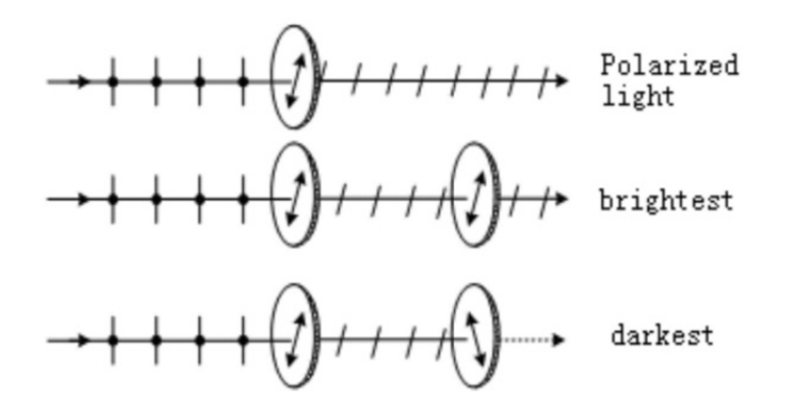
\includegraphics[scale=1.0]{polar.png}
\caption{Change in the brightness of the light depends on the mutual orientation of the polarizer and the analyzer.}\label{fig.Malus}
\end{figure}

\subsection{Generation of Elliptically and Circularly Polarized Light. Half-wave and Quarter-wave Plates}

If a linearly polarized light is incident morally on a crystal plate whose surface is parallel to its optical axis, and the angle between the polarizing axis and the optical axis of the plate is $\alpha$, then the linearly polarized light is resolved into two waves: an e-wave with the oscillation direction parallel to the optical axis of the plate (extraordinary axis) and an o-wave whose oscillation direction is perpendicular to the optical axis (ordinary axis). They propagate in the same direction, but with different speeds. The resulting optical path difference over the thickness d of the plate is
$$\Delta = (n_\text{e} - n_\text{o})d,$$
and, consequently, the phase difference
$$\delta = \frac{2\pi}{\lambda}(n_\text{e} - n_\text{o})d,$$ 
where $\lambda$ is the wavelength, $n_\text{e}$ is the refractive index for the extraordinary axis, and $n_\text{o}$ is the refractive index for the ordinary axis. In a so-called positive crystal $\delta > 0$, whereas in a negative one $\delta < 0$.

As shown in Figure 4, when the light propagates through the crystal plate, the two components of the light vector are
\begin{align*}
E_x &= A_\text{o}\cos\omega t\\
E_y &= A_\text{e}\cos(\omega t + \delta),
\end{align*}
where $A_\text{e} = A\cos\alpha$, $A_\text{o} = A\sin\alpha$. Eliminating time from the above equations one obtains
\begin{equation}\label{eqE}
\frac{E_x^2}{A_\text{o}^2} + \frac{E_y^2}{A_\text{e}^2} - 2\frac{E_xE_y}{A_\text{o}A_\text{e}}\cos \delta = \sin^2\delta,
\end{equation}
which is the equation of an ellipse.

\begin{figure}[H]\centering
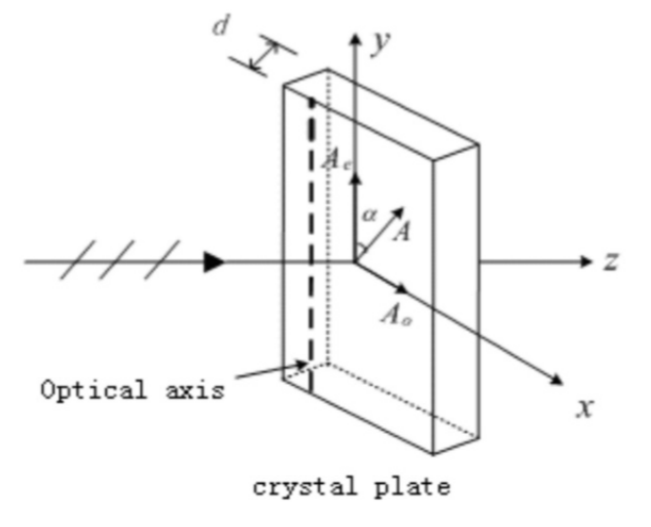
\includegraphics[scale=1.0]{crystal.png}
\caption{Linearly polarized light passing through a waveplate.}\label{FigCrystal}
\end{figure}

When the thickness of the plate changes, the optical path difference changes as well. Some cases of particular interest, are discussed below: 

\begin{enumerate}[$\blacktriangleright$]
\item If $\Delta = k\lambda$, where $k = 0,1,2,...,$ the phase difference $\delta = 0$, and Eq. (\ref{eqE}) reduces to
$$E_y = \frac{A_\text{e}}{A_\text{o}}E_x,$$
which is a linear equation. Hence the transmitted light is linearly polarized with the oscillation direction remaining unchanged. A waveplate that satisfies this condition is called a \textit{full-wave} plate. The light goes through a full-wave plate without changing its polarization state.
\item If $\Delta = (2k + 1)\lambda/2$, where $k = 0,1,2,...,$ the phase difference $\delta = \pi$, and Eq. (\ref{eqE}) simplifies to
$$E_y = -\frac{A_\text{e}}{A_\text{o}}E_x.$$  
The transmitted light is also linearly polarized with the polarization axis rotated by the angle of $2\alpha$. A waveplate that satisfies the condition is called \textit{1/2-wave plate} or \textit{half-wave plate}. When a polarized light passes through a half-wave plate, its polarization axis gets rotated by an angle $2\alpha$. If $\alpha = \pi/4$, then the polarization axis of the transmitted light is perpendicular to that of the incident light.
\item Finally, if $\Delta = (2k + 1)\lambda/4$, where $k = 0,1,2,...,$ the phase difference $\delta = \pm\pi/2$, and Eq. (\ref{eqE}) transforms into
$$\frac{E_x^2}{A_\text{o}^2} \pm \frac{E_y^2}{A_\text{e}^2} = 1.$$
The transmitted light is elliptically polarized with a waveplate that satisfies the above condition is called a \textit{1/4-wave plate} or a \textit{quarter-waveplate} and is an important optical element in many polarization experiments.
\end{enumerate}

If $A_\text{e} = A_\text{o} = A$, then $E^2_x +E^2_y = A^2$, and the transmitted light is circularly polarized. Since the amplitudes of the \textit{o}-wave and the \textit{e}-wave are both functions of $\alpha$, the polarization state after passing through a 1/4-wave plate will vary, depending on the angle: 

\begin{enumerate}[$\blacktriangleright$]
\item if $\alpha = 0$, the transmitted light is linearly polarized with the polarization axis parallel to the optical axis of the 1/4-wave plate; 
\item if $\alpha = \pi/2$, the transmitted light is linearly polarized with the polarization axis perpendicular to the optical axis of the 1/4-wave plate; 
\item if $\alpha = \pi/4$, the transmitted light is circularly polarized; 
\item otherwise, the transmitted light is elliptically polarized.
\end{enumerate}

\section{Experimental Setup}

The experimental setup in this lab consists of a laser, a silicon photo-cell, a UT51 digital universal meter, two polarizers, a 1/2-wave plate, a 1/4-wave plate. 

The precision of the devices is shown in Table \ref{tablePresicion}.

\begin{table}[H]
\centering
\begin{tabular}{ccc}
\toprule
Instrument & Measurement Quantity & Uncertainty\\
\midrule
Scale on the element & Angle $\theta$ & $\pm2^\circ$\\
 Universal meter & Current $I$ & $\pm0.001\mu A$ or $\pm0.01\mu A$\\
\bottomrule
\end{tabular}
\caption{Precision of the measurement instruments.}\label{tablePresicion}
\end{table}

\section{Measurement Procedure}

\subsection{Apparatus Adjustment}
\begin{enumerate}
\item Adjust the laser and the photo-cell so that the light can pass through the $\phi$ 6.0 aperture
\item Fix the laser at one of the ends of the bench and place the glass sheet and lens in front of it. Adjust the position so that the light passes through the center of the lens. Make sure that the light spot on the lens won't change significantly if the glass sheet moves along the bench.
\item Remove the glass sheet. Set the digital universal meter in the appropriate mode and range.
\end{enumerate}

\subsection{Demonstration of Malus' Law}
\begin{enumerate}
\item Place an analyzer between the polarizer and the photo-cell as is shown in Figure \ref{fig.setup}.
\item Adjust the angle of the analyzer until the electric current reaches its minimum. This position is considered to be $\theta = 90^\circ$.
\item Rotate the analyzer from $90^\circ$ to $0^\circ$ and measure the corresponding current $I$ every $5^\circ$.
\item Plot the graph $I/I_0$ vs. $\cos^2\theta$ and perform linear fitting.
\end{enumerate}

\begin{figure}
\centering
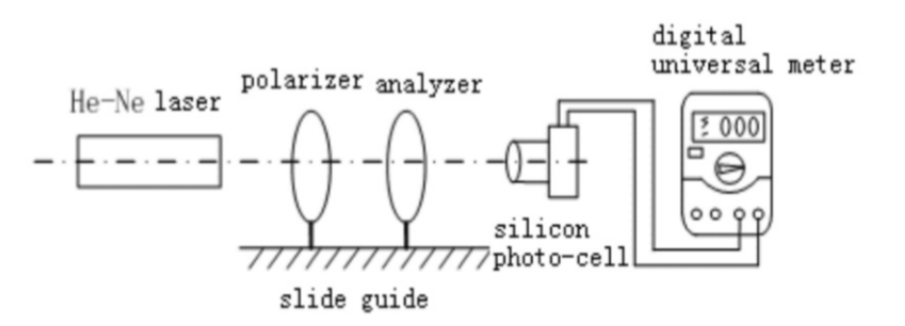
\includegraphics[scale=1]{setup.PNG}
\caption{Experimental setup for a demonstration of Malus’ law.}\label{fig.setup}
\end{figure}

\subsection{Linearly Polarized Light and the Half-wave Plate}
\begin{enumerate}
\item Place the 1/2-wave plate between the polarizer and the analyzer. 
\item Rotate the 1/2-wave plate to make the light extinction appear again and set this position as the initial position.
\item Rotate the 1/2-wave plate for $\alpha = 10^\circ$ from the initial position and rotate the analyzer to make the light extinction appear again, record the angle of rotation $\Delta\theta$. Repeat this operation for 8 times, where  $\Delta\theta$ becomes $90^{\circ}$ at the end.
\item Plot the graph $\Delta\theta$ vs. $\theta$.
\end{enumerate}

\subsection{Circularly and Elliptically Polarized Light and the 1/4-wave Plate}
\begin{enumerate}
\item Maintain the previous setup. Replace the 1/2-wave plate with a 1/4-wave plate and rotate it to make the light extinction appear and set this position as the initial position. At this point $\alpha = 0^\circ$. Then rotate the 1/4-wave plate and observe the change in the light intensity.
\item Rotate the analyzer for $360^\circ$  for every $10^{\circ}$,  and record the light intensity indicated by the current $I$ in the table.
\item Rotate the 1/4-wave plate for $20^\circ$, repeat Step 2.
\item Rotate the 1/4-wave plate for $45^\circ$, repeat Step 2.
\item Rotate the 1/4-wave plate for $70^\circ$. Rotate the analyzer and record its position and the magnitude of the current when the light intensity reaches a maximum.
\item Plot the curves between the rotation angle of the analyzer and the light amplitude in polar coordinates. Normalize the amplitude by its maximum value. Mark the position recorded in Step 5 and compare it with the data recorded. 
\item Compare the data with the circular polarization, plot a linear fit to the data when the angle is $45^\circ$.
\end{enumerate}



		\section{Result}
\subsection{Demonstration of Malus' Law}
In this part, the current corresponding to different angles of analyzer are measured. And the measurement data are presented in Table \ref{tab.Malus}. 

Then,  corresponding $\cos^2\theta$ and $I/I_0$ can be calculated. 
Take the first set of data as an calculation example.
$$\cos^2\theta = \cos^2(0 \times \frac{\pi}{180}) = 1 \pm 0,$$
$$\frac{I}{I_0} = \frac{1.037}{1.037} = 1.0000 \pm 0.0013.$$
The rest of the results are shown in Table \ref{tab.Malus2}.

\begin{table}[]
\centering
\begin{tabular}{cc}
\toprule
\multicolumn{2}{c}{Maximum   Electric Current $I_0$:} \\ 
\multicolumn{2}{c}{$2.00 \pm ~ 0.01 [\mu A]$} \\ \midrule
$\theta~[^{\circ}]$                & $I [\mu A]~\pm~0.01 [\mu A]$               \\ \midrule
0                                  & 2.00                                       \\
5                                  & 1.97                                       \\
10                                 & 1.97                                       \\
15                                 & 1.92                                       \\
20                                 & 1.84                                       \\
25                                 & 1.73                                       \\
30                                 & 1.60                                       \\
35                                 & 1.46                                       \\
40                                 & 1.33                                       \\
45                                 & 1.18                                       \\
50                                 & 1.01                                       \\
55                                 & 0.82                                       \\
60                                 & 0.69                                       \\
65                                 & 0.48                                       \\
70                                 & 0.34                                       \\
75                                 & 0.23                                       \\
80                                 & 0.11                                       \\
85                                 & 0.04                                       \\
90                                 & 0.01                                      \\ \bottomrule
\end{tabular}
\caption{Measurement data for Malus' law demonstration.}
\label{tab.Malus}
\end{table}


\begin{table}[H]
\centering
\begin{tabular}{cccc}
\toprule
\multicolumn{1}{l}{$cos^2(\theta)$} & \multicolumn{1}{l}{$\mu_{cos^2(\theta)}$} & \multicolumn{1}{l}{$I/I_0$} & \multicolumn{1}{l}{$\mu_{I/I_0}$} \\ \midrule
1 & 0 & 1.000 & 0.007 \\
0.992 & 0.006 & 0.985 & 0.007 \\
0.970 & 0.012 & 0.985 & 0.007 \\
0.933 & 0.017 & 0.960 & 0.007 \\
0.88 & 0.02 & 0.920 & 0.007 \\
0.82 & 0.03 & 0.865 & 0.007 \\
0.75 & 0.03 & 0.800 & 0.006 \\
0.67 & 0.03 & 0.730 & 0.006 \\
0.59 & 0.03 & 0.665 & 0.006 \\
0.50 & 0.03 & 0.590 & 0.006 \\
0.41 & 0.03 & 0.505 & 0.006 \\
0.33 & 0.03 & 0.410 & 0.005 \\
0.25 & 0.03 & 0.345 & 0.005 \\
0.18 & 0.03 & 0.240 & 0.005 \\
0.12 & 0.02 & 0.170 & 0.005 \\
0.067 & 0.017 & 0.115 & 0.005 \\
0.030 & 0.012 & 0.055 & 0.005 \\
0.008 & 0.006 & 0.020 & 0.005 \\
0 & 0 & 0.005 & 0.005 \\ \bottomrule
\end{tabular}
\caption{Result for $\cos^2\theta$ and $I/I_0$.}
\label{tab.Malus2}
\end{table}



\begin{figure}[H]
\centering
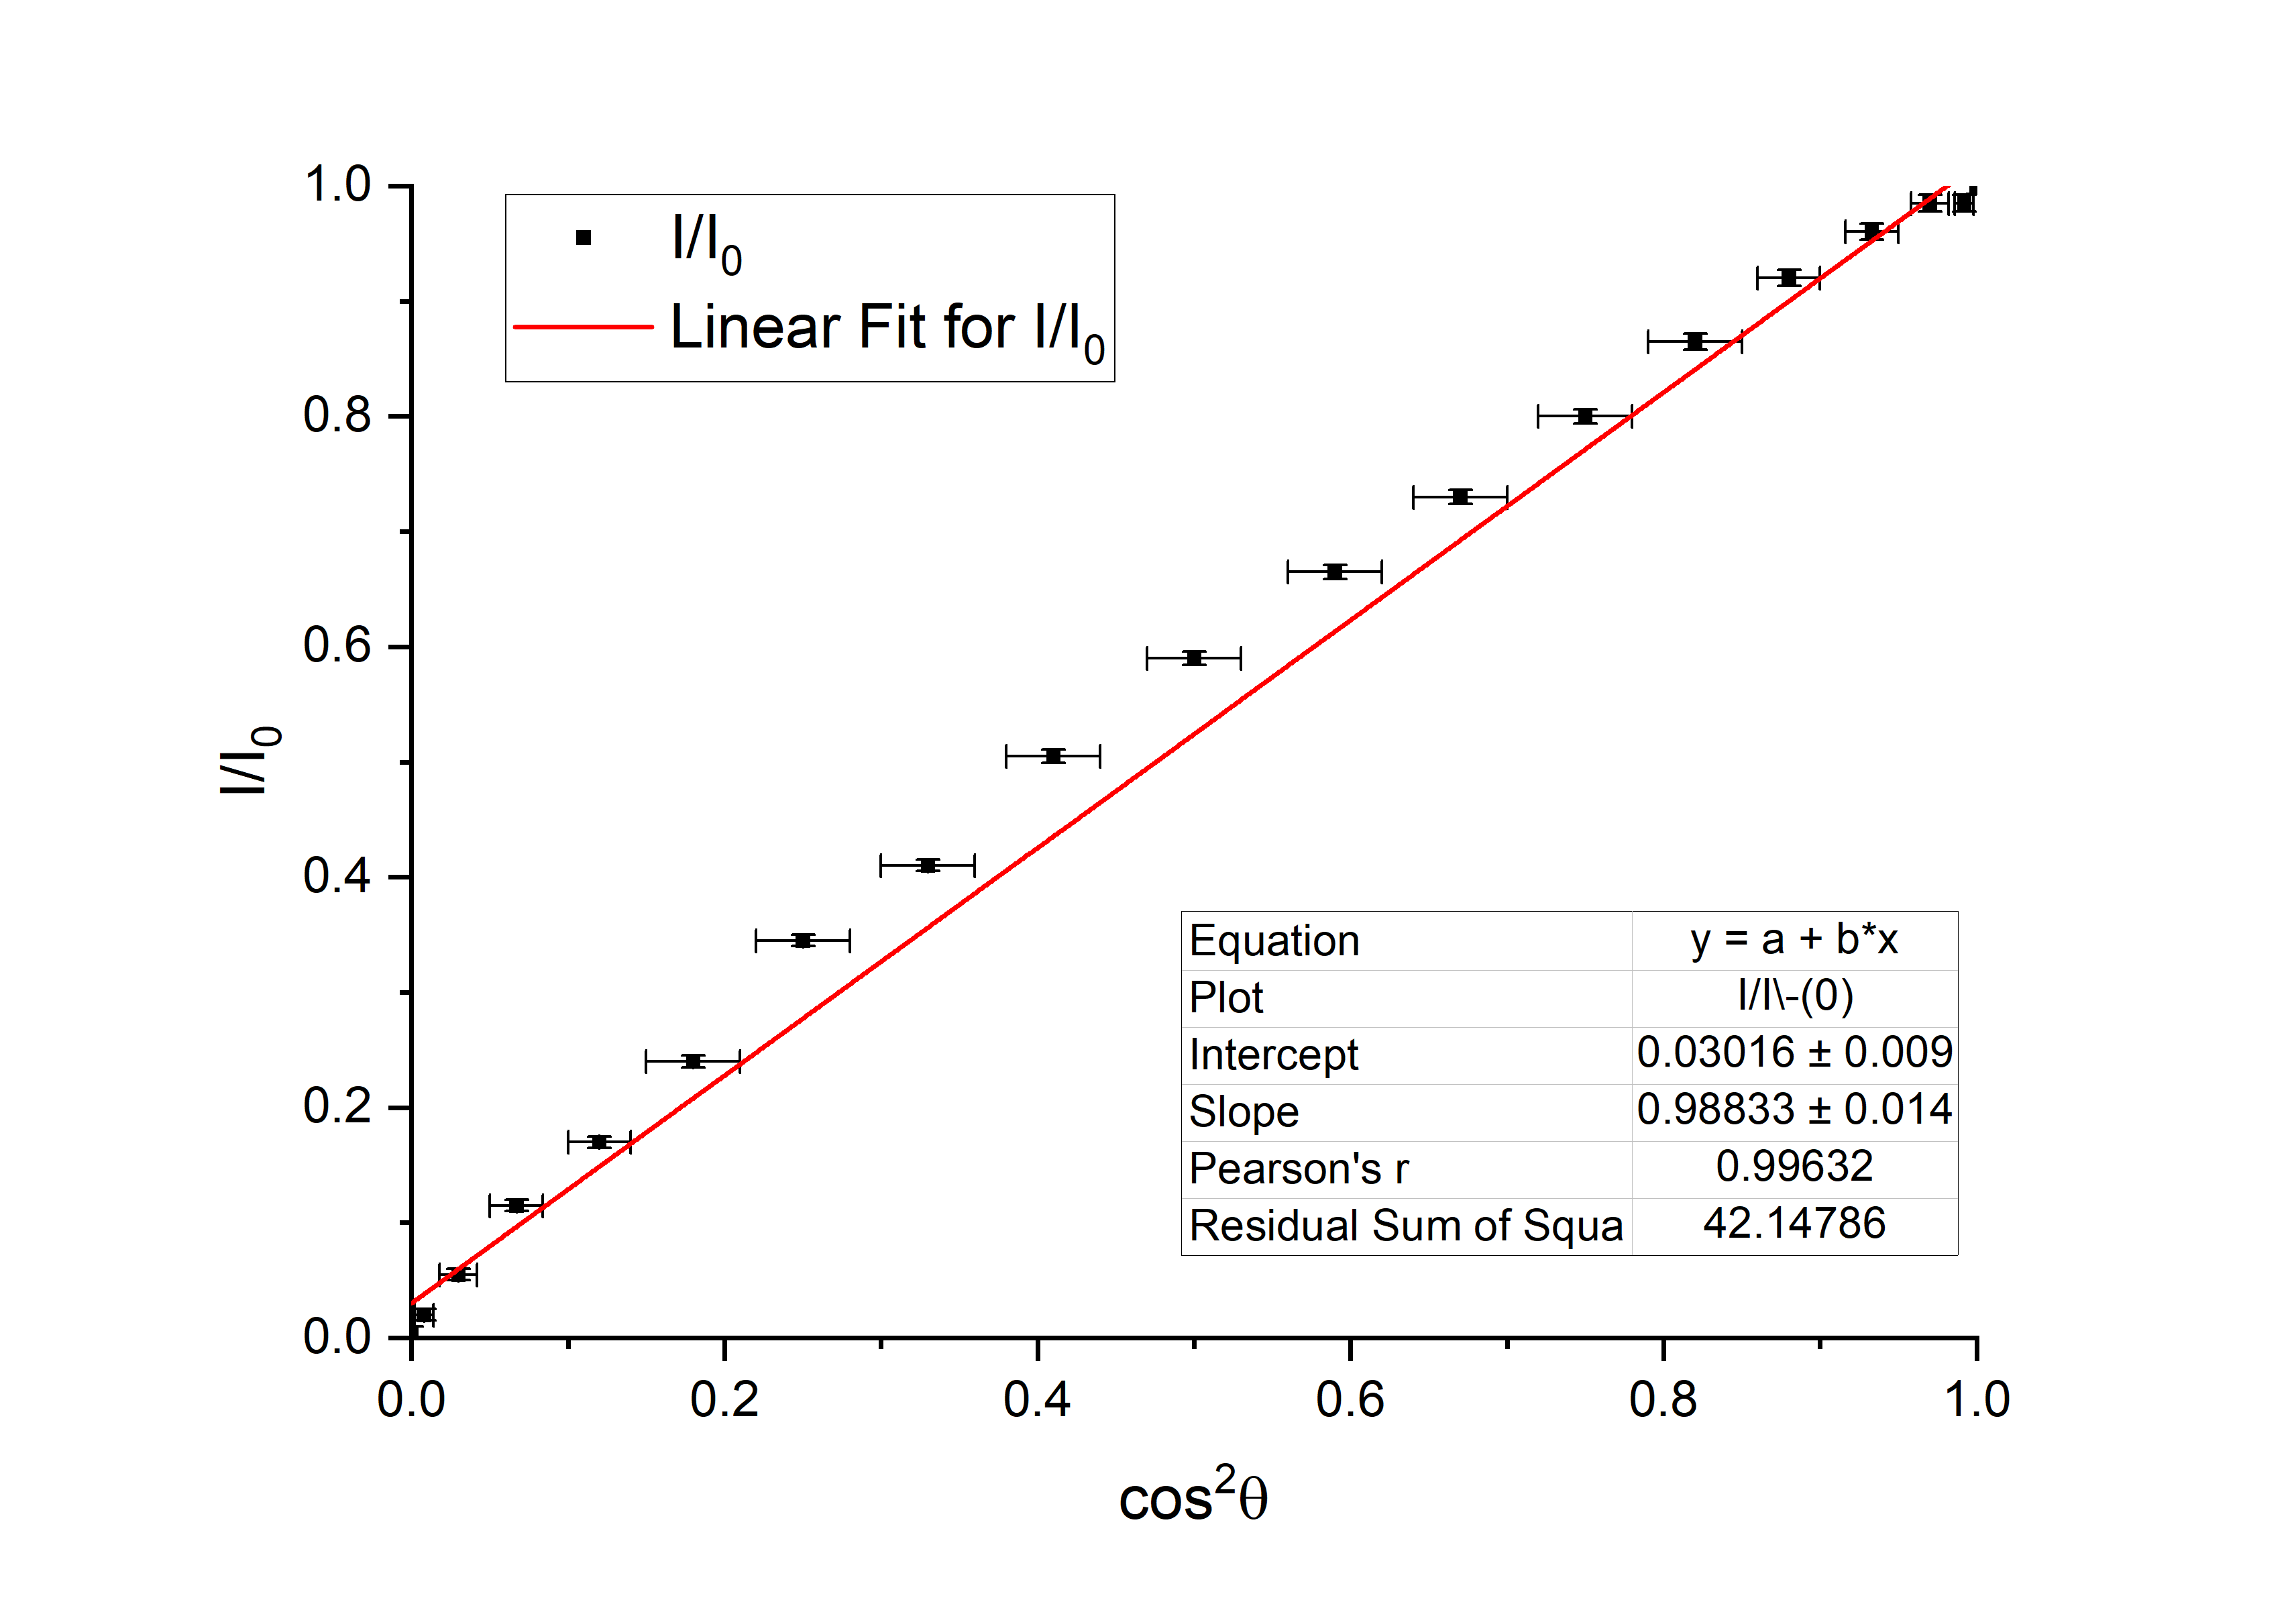
\includegraphics[scale=0.6]{1}
\caption{Linear fit for $I/I_0$ v.s $cos^2\theta$}\label{fig.cos-I}
\end{figure}

Then, a linear fit of the plot $I/I_0$ vs. $\cos^2\theta$ are performed (Figure \ref{fig.cos-I}). The slope of the linear fitting is 0.988 $\pm$ 0.014. And the Pearson's r is 0.996, which is very close to 1.

\subsection{Linearly Polarized Light and the Half-wave Plate}

In this part, the rotation angles of the 1/2 plate and the analyzer are measured. The measurement data are presented in Table \ref{Table1/2}. 

\begin{table}[H]\centering
\begin{tabular}{cc}
\toprule
Rotation angle of the 1/2-wave plate $[^\circ] \pm 2[^\circ]$ & Rotation angle of the analyzer $[^\circ] \pm 2[^\circ]$\\
\midrule 
initial & 0 \\
10 & 18 \\
20 & 36 \\
30 & 56 \\
40 & 74 \\
50 & 92 \\
60 & 112 \\
70 & 132 \\
80 & 152 \\
90 & 172 \\
\bottomrule
\end{tabular}
\caption{Measurement data for the 1/2-wave plate.}\label{Table1/2}
\end{table}

To find the relation between $\Delta\theta$ and $\theta$, the data are plotted in Figure \ref{fig.theta} and linear fit is performed. The slope of the linear fit is $1.91 \pm 0.05$ with Pearson's r=0.999.

\begin{figure}[H]\centering
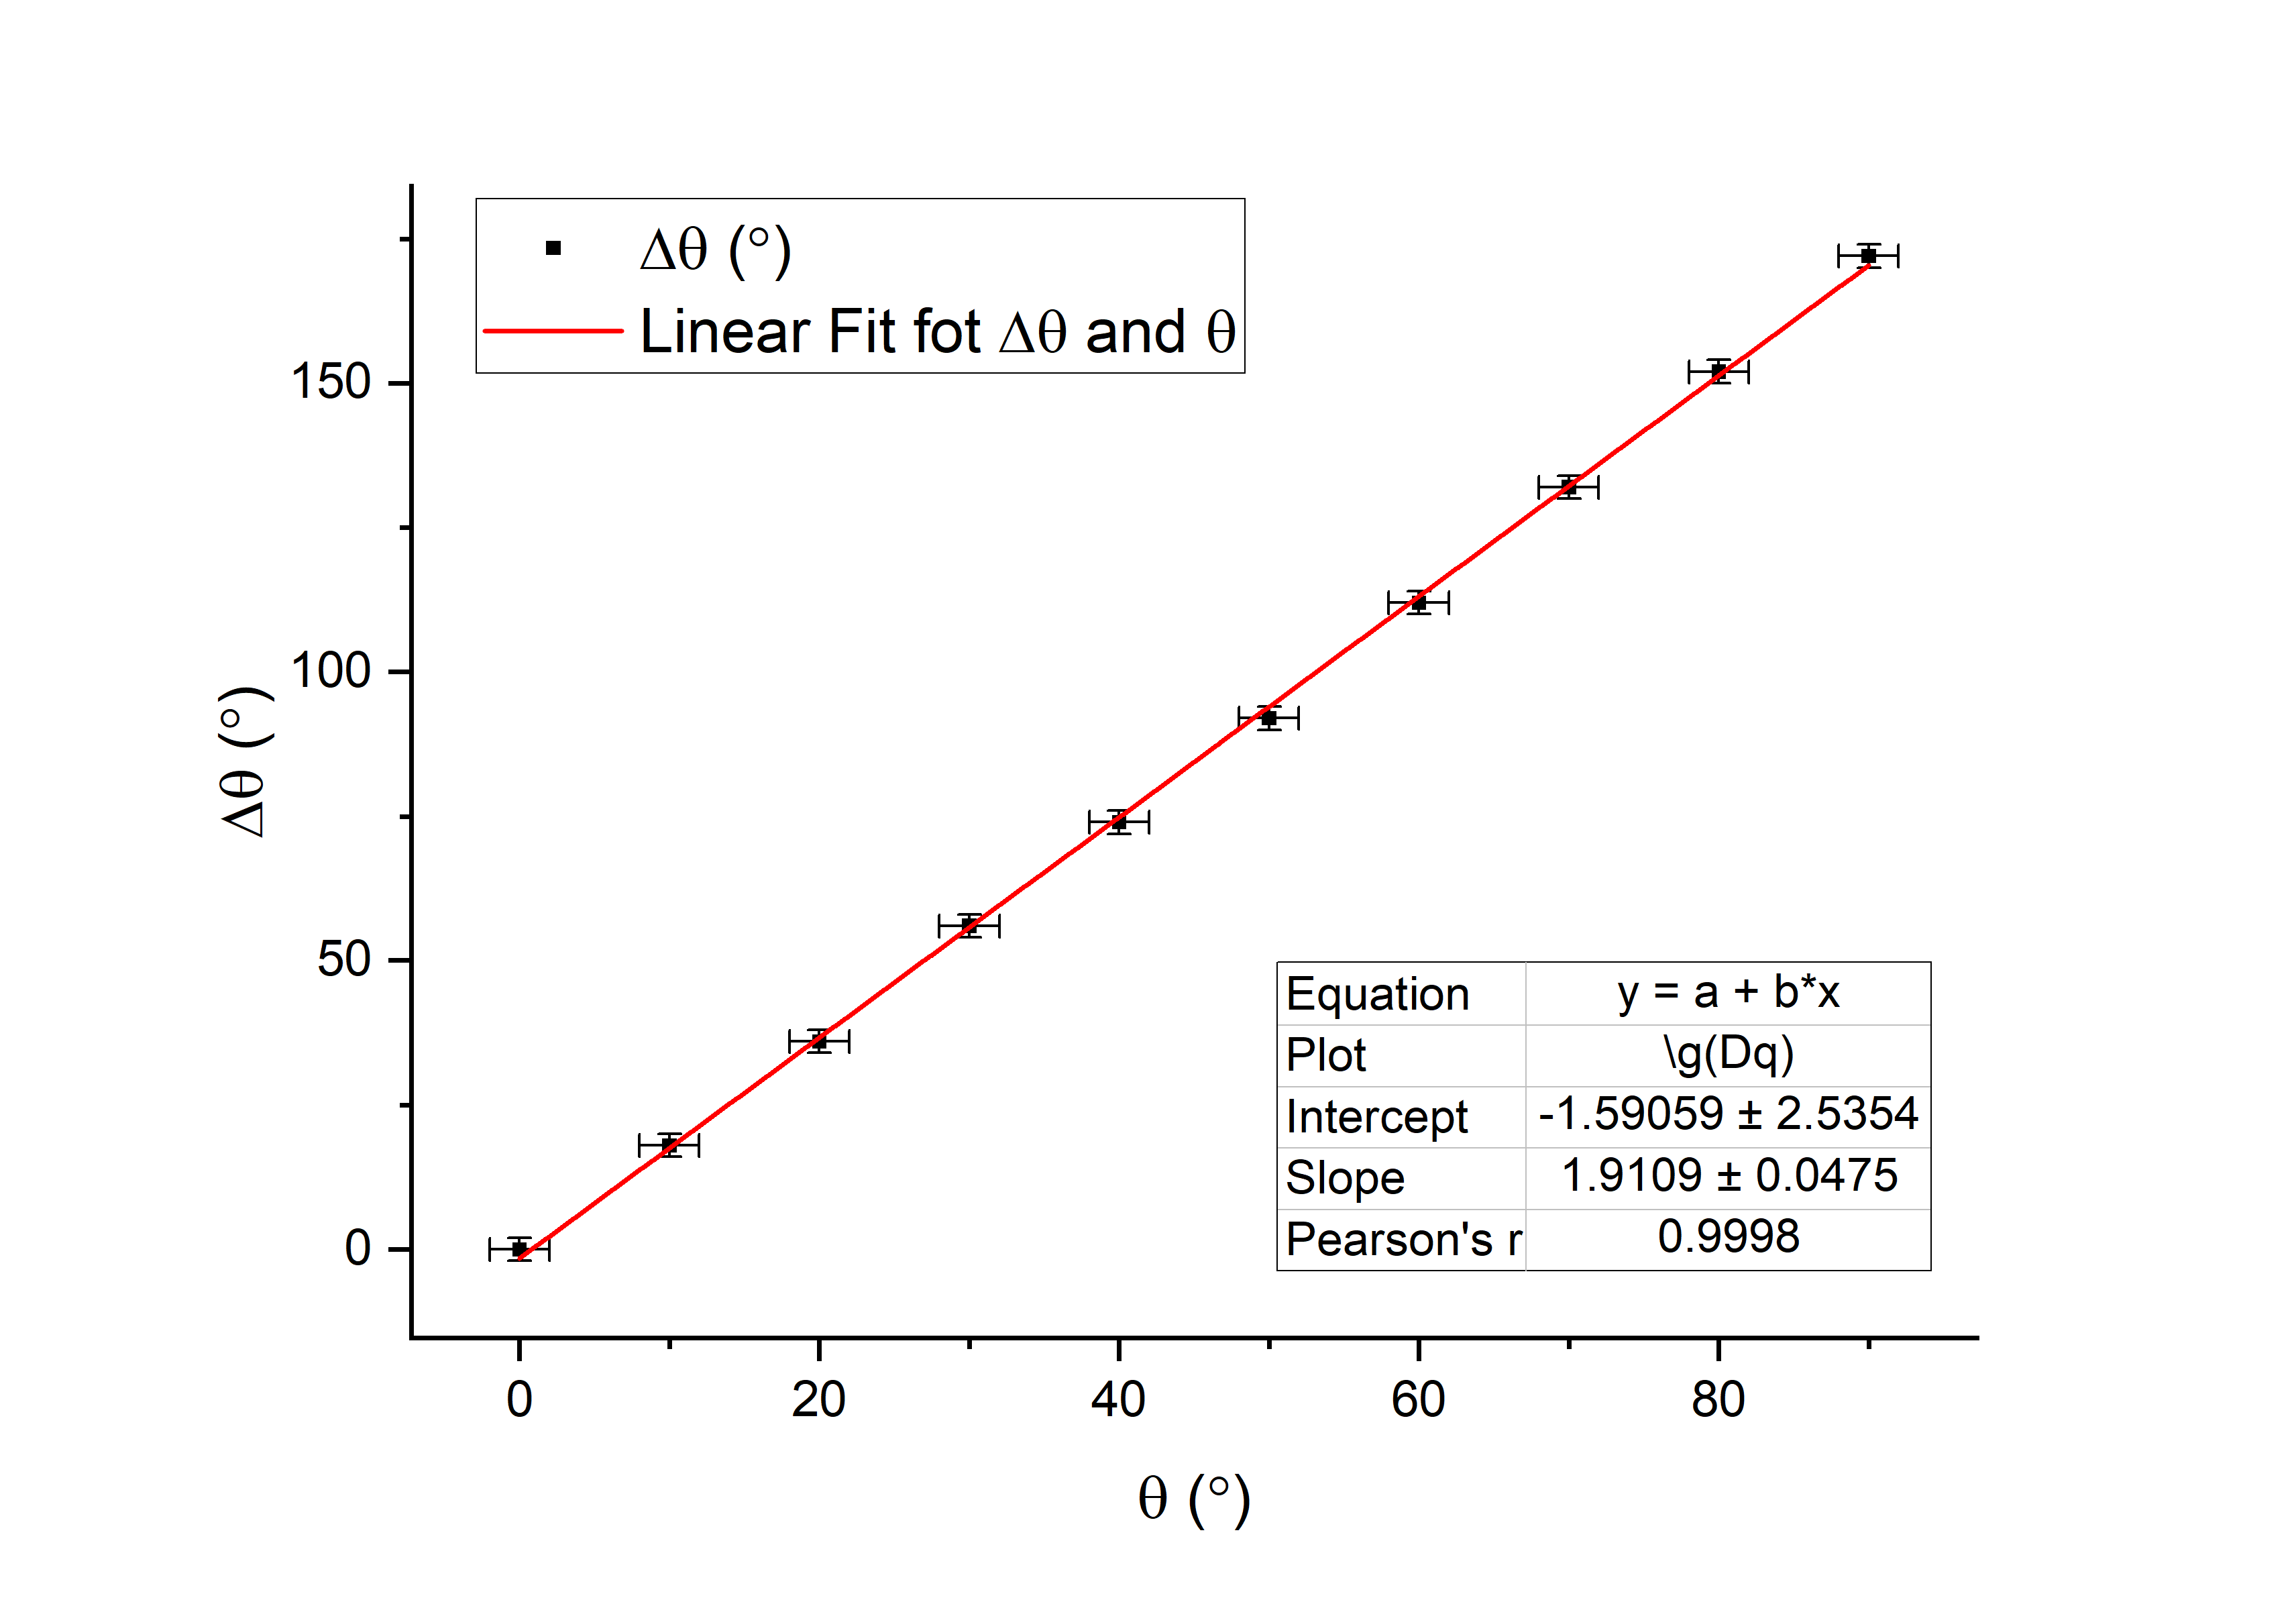
\includegraphics[scale=0.6]{2.png}
\caption{Linear fit of $\Delta\theta$ vs. $\theta$.}\label{fig.theta}
\end{figure}

\begin{enumerate}
\item When the half-wave plate rotates for 360$^\circ$, 4 times of light extinction are observed.
\item When the analyzer rotates for 360$^\circ$, 2 times of light extinction during the analyzer rotating 360$^\circ$. 
\item Explanation: after the light passes through the 1/2-wave plate, the polarization axis is rotated by twice of the origin angle.
\end{enumerate}

	\subsection{Circularly and Elliptically Polarized Light and the 1/4-wave Plate}

			\subsubsection{Rotation Angle: 0$^\circ$} \label{sec:0degree}

The measurement data for 0$^\circ$ rotation angle of 1/4-wave plate are presented in Table \ref{Table1/40}. 

\begin{table}[H]\centering
\begin{tabular}{cc||cc}
\toprule
\multicolumn{4}{c}{Rotation angle of 1/4-wave plate: 0$^\circ$}\\
\toprule
\multicolumn{2}{c}{Maximum Electric Current $I_0$} & \multicolumn{2}{c}{1.50 $\pm$ 0.01 [$\mu$A]}\\
\midrule
$\theta\,\,[^\circ] \pm 2[^\circ]$ & $I\,\,[\mu\text{A}] \pm 0.01\,\,[\mu\text{A}]$ & $\theta\,\,[^\circ] \pm 2[^\circ]$ & $I\,\,[\mu\text{A}] \pm 0.01\,\,[\mu\text{A}]$\\
\midrule
0 & 0.02 & 180 & 0.02 \\
10 & 0.07 & 190 & 0.08 \\
20 & 0.22 & 200 & 0.20 \\
30 & 0.43 & 210 & 0.44 \\
40 & 0.69 & 220 & 0.69 \\
50 & 0.93 & 230 & 0.94 \\
60 & 1.15 & 240 & 1.10 \\
70 & 1.33 & 250 & 1.31 \\
80 & 1.38 & 260 & 1.43 \\
90 & 1.42 & 270 & 1.50 \\
100 & 1.35 & 280 & 1.39 \\
110 & 1.19 & 290 & 1.25 \\
120 & 0.99 & 300 & 1.06 \\
130 & 0.82 & 310 & 0.85 \\
140 & 0.57 & 320 & 0.60 \\
150 & 0.34 & 330 & 0.35 \\
160 & 0.17 & 340 & 0.15 \\
170 & 0.05 & 350 & 0.02 \\ 
\bottomrule
\end{tabular}
\caption{Measurement data for the 1/4-wave plate (rotation angle 0$^\circ$).}\label{Table1/40}
\end{table}

As described in the procedure part, $\sqrt{I/I_0}$ is calculated. Take the first set of data as an example,
$$\sqrt{\frac{I}{I_0}} = \sqrt{\frac{0.02}{1.50}} = 0.12 \pm 0.08.$$
Perform similar calculations to each of the other sets of data and the results are presented in Table \ref{TableSqrt}.

\begin{table}[H]\centering
\begin{tabular}{ccc||ccc}
\toprule
$\theta\,\,[^\circ] \pm 2[^\circ]$ & $\sqrt{I/I_0}$ & $\mu_{\sqrt{I/I_0}}$ & $\theta\,\,[^\circ] \pm 2[^\circ]$ & $\sqrt{I/I_0}$ & $\mu_{\sqrt{I/I_0}}$ \\
\midrule
0 & 0.12 & 0.03 & 180 & 0.12 & 0.03 \\
10 & 0.22 & 0.015 & 190 & 0.231 & 0.014 \\
20 & 0.383 & 0.009 & 200 & 0.365 & 0.009 \\
30 & 0.535 & 0.006 & 210 & 0.542 & 0.006 \\
40 & 0.678 & 0.005 & 220 & 0.678 & 0.005 \\
50 & 0.787 & 0.005 & 230 & 0.792 & 0.005 \\
60 & 0.876 & 0.005 & 240 & 0.856 & 0.005 \\
70 & 0.942 & 0.005 & 250 & 0.935 & 0.005 \\
80 & 0.959 & 0.005 & 260 & 0.976 & 0.005 \\
90 & 0.973 & 0.005 & 270 & 1.000 & 0.005 \\
100 & 0.949 & 0.005 & 280 & 0.963 & 0.005 \\
110 & 0.891 & 0.005 & 290 & 0.913 & 0.005 \\
120 & 0.812 & 0.005 & 300 & 0.841 & 0.005 \\
130 & 0.739 & 0.005 & 310 & 0.753 & 0.005 \\
140 & 0.616 & 0.006 & 320 & 0.632 & 0.006 \\
150 & 0.476 & 0.007 & 330 & 0.483 & 0.007 \\
160 & 0.337 & 0.010 & 340 & 0.316 & 0.011 \\
170 & 0.18 & 0.02 & 350 & 0.12 & 0.03  \\
\bottomrule
\end{tabular}
\caption{Results for $\sqrt{I/I_0}$ when rotation angle is 0$^\circ$.}\label{TableSqrt}
\end{table}

Then the relationship of $\sqrt{I/I_0}$ and $\theta$ are plotted in polar coordinate (Figure \ref{Fig0}).

\begin{figure}[H]\centering
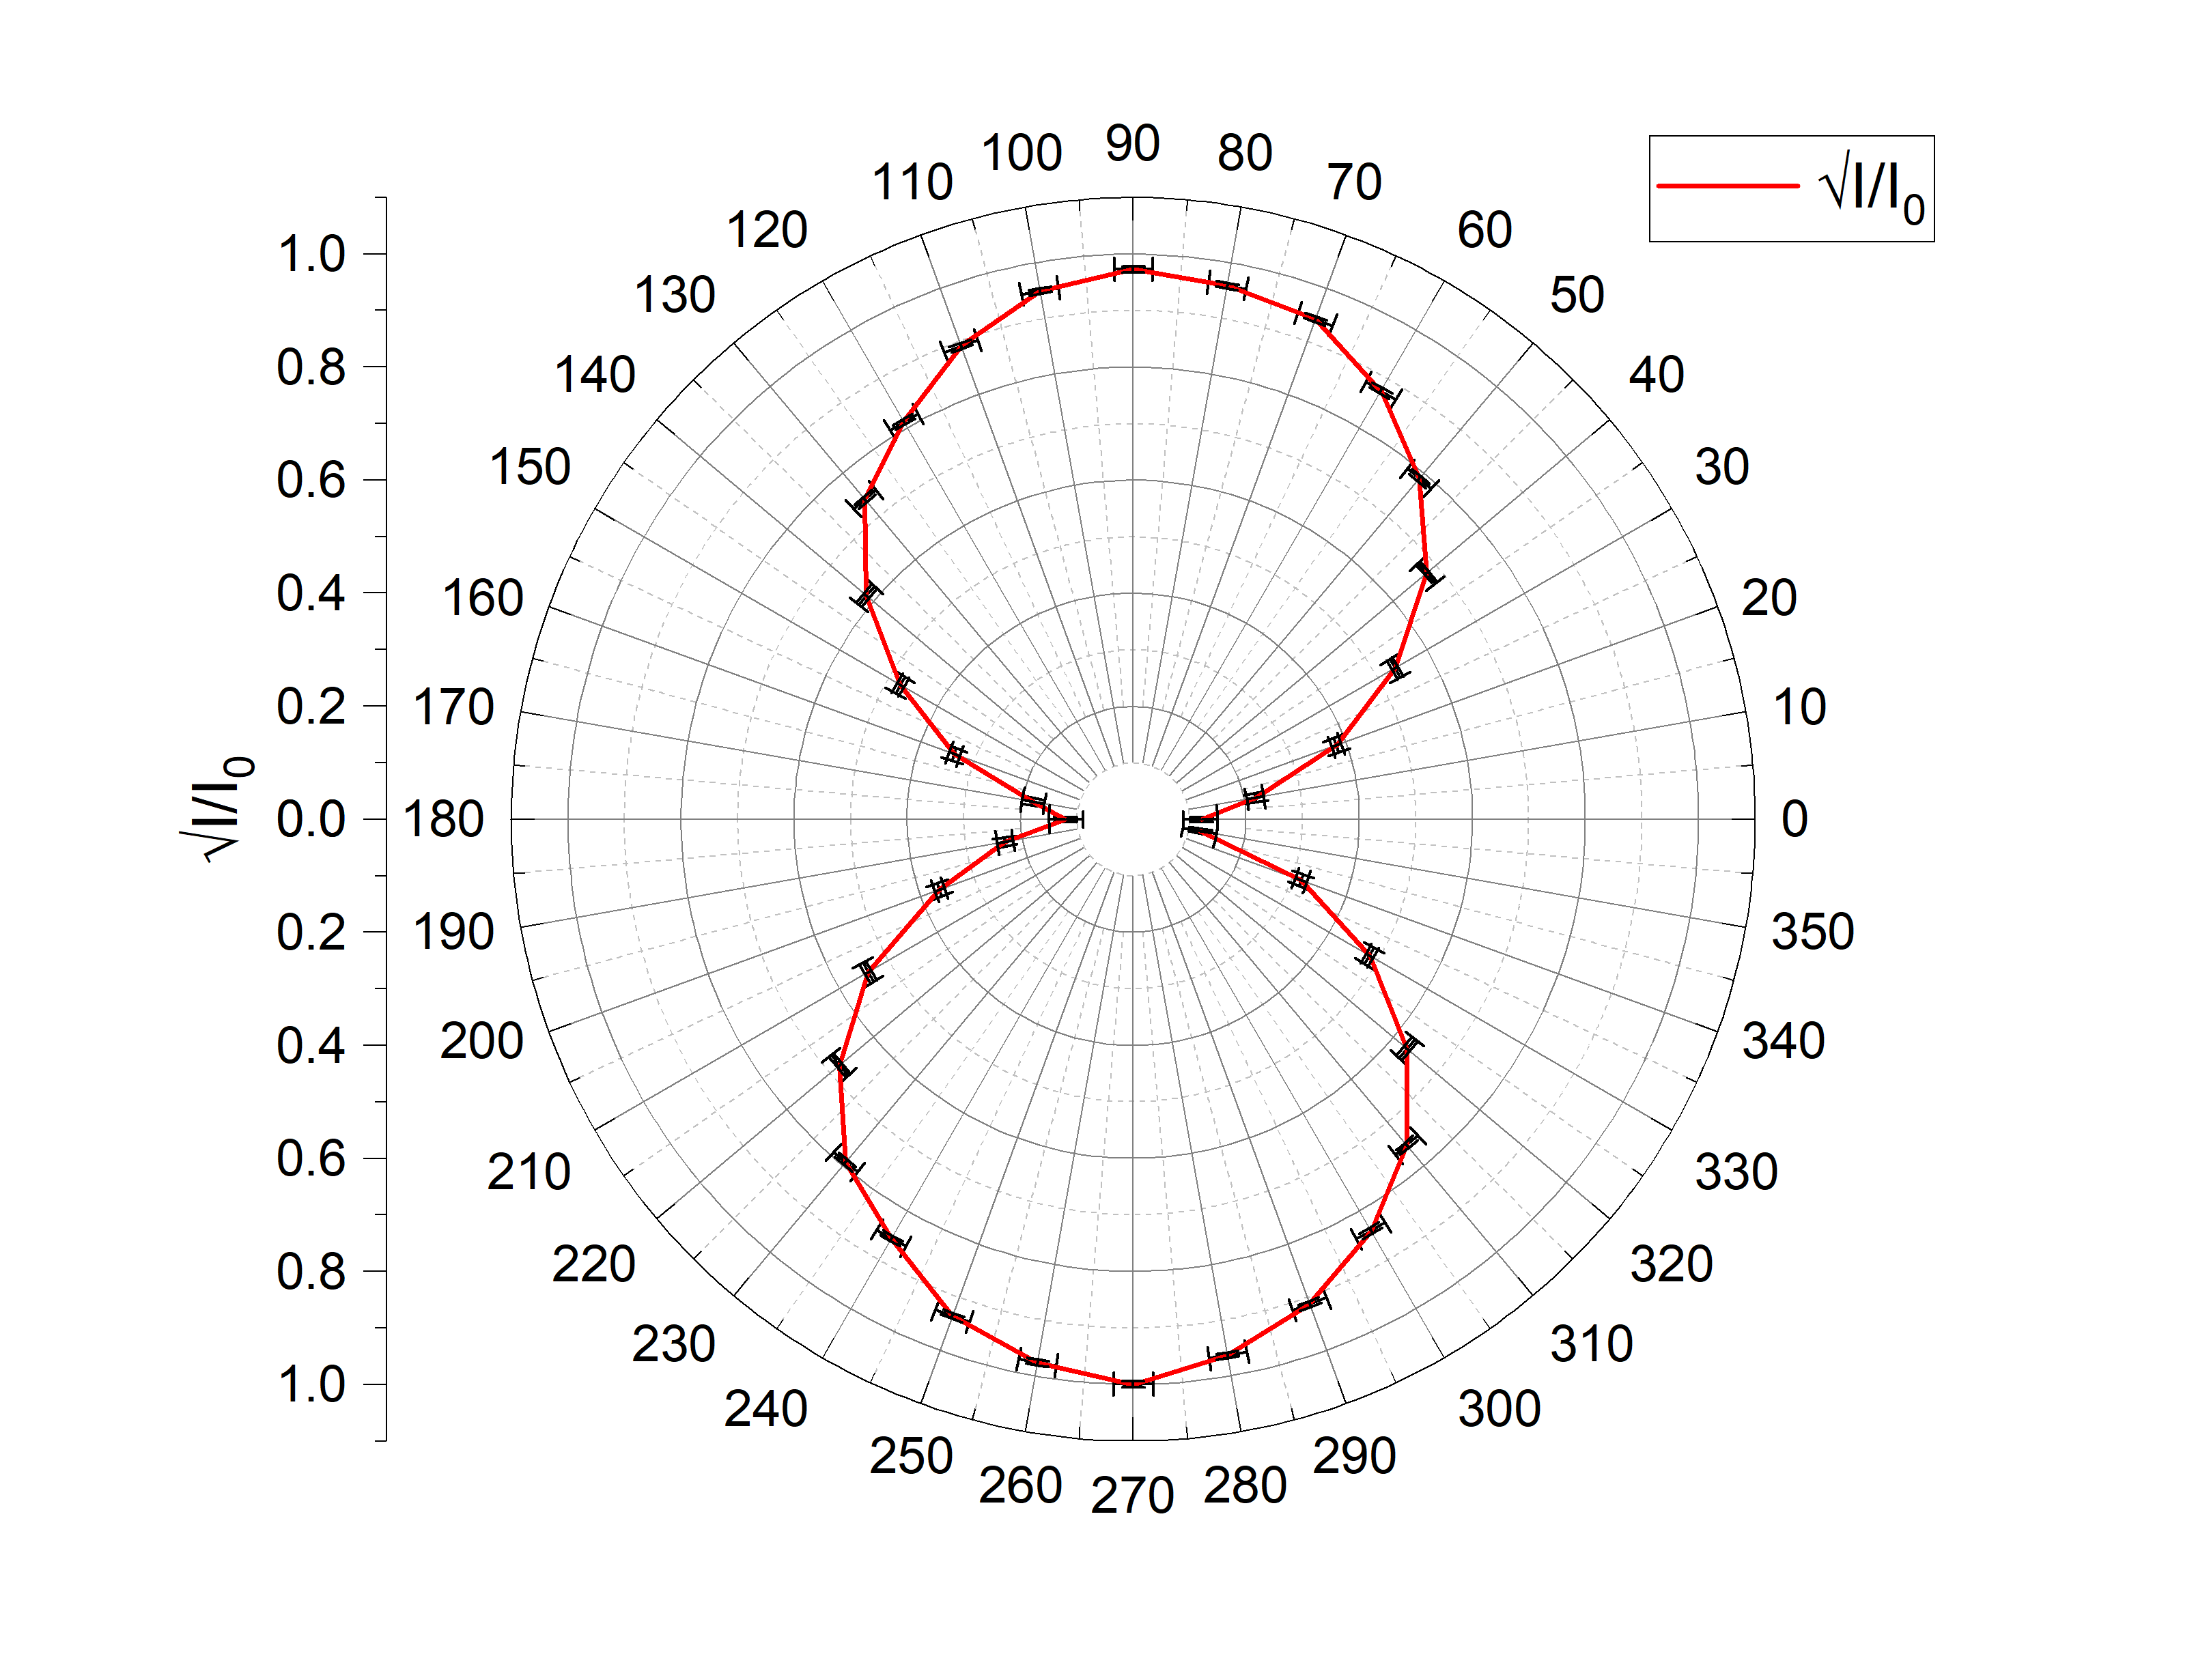
\includegraphics[scale=0.6]{3.png}
\caption{$\sqrt{I/I_0}$ vs. $\theta$ relation in polar coordinate when rotation angle is 0$^\circ$.}\label{Fig0}
\end{figure}

\newpage

\subsubsection{Rotation Angle: 20$^\circ$}

The measurement data for 20$^\circ$ rotation angle of 1/4-wave plate are shown in Table \ref{Table1/420}.  

\begin{table}[H]\centering
\begin{tabular}{cc||cc}
\multicolumn{4}{c}{Rotation angle of 1/4-wave plate: 20$^\circ$}\\
\toprule
\multicolumn{2}{c}{Maximum Electric Current $I_0$} & \multicolumn{2}{c}{0.707 $\pm$ 0.001 [$\mu$A]}\\
\midrule
$\theta\,\,[^\circ] \pm 2[^\circ]$ & $I\,\,[\mu\text{A}] \pm 0.001\,\,[\mu\text{A}]$ & $\theta\,\,[^\circ] \pm 2[^\circ]$ & $I\,\,[\mu\text{A}] \pm 0.001\,\,[\mu\text{A}]$\\
\midrule
0 & 0.19 & 180 & 0.18 \\
10 & 0.22 & 190 & 0.22 \\
20 & 0.32 & 200 & 0.31 \\
30 & 0.44 & 210 & 0.45 \\
40 & 0.60 & 220 & 0.61 \\
50 & 0.77 & 230 & 0.76 \\
60 & 0.89 & 240 & 0.93 \\
70 & 1.03 & 250 & 1.02 \\
80 & 1.09 & 260 & 1.16 \\
90 & 1.11 & 270 & 1.19 \\
100 & 1.07 & 280 & 1.17 \\
110 & 1.03 & 290 & 1.08 \\
120 & 0.92 & 300 & 0.97 \\
130 & 0.78 & 310 & 0.80 \\
140 & 0.61 & 320 & 0.60 \\
150 & 0.45 & 330 & 0.43 \\
160 & 0.31 & 340 & 0.31 \\
170 & 0.21 & 350 & 0.23 \\
\bottomrule
\end{tabular}
\caption{Measurement data for the 1/4-wave plate (rotation angle 20$^\circ$).}\label{Table1/420}
\end{table}

Similarly, $\sqrt{I/I_0}$ is calculated and the results are presented in Table \ref{TableSqrt20}.

\begin{table}[H]\centering
\begin{tabular}{ccc||ccc}
\toprule
$\theta\,\,[^\circ] \pm 2[^\circ]$ & $\sqrt{I/I_0}$ & $\mu_{\sqrt{I/I_0}}$ & $\theta\,\,[^\circ] \pm 2[^\circ]$ & $\sqrt{I/I_0}$ & $\mu_{\sqrt{I/I_0}}$ \\
\midrule
0 & 0.400 & 0.009 & 180 & 0.389 & 0.009 \\
10 & 0.430 & 0.008 & 190 & 0.430 & 0.008 \\
20 & 0.519 & 0.005 & 200 & 0.510 & 0.005 \\
30 & 0.608 & 0.004 & 210 & 0.615 & 0.004 \\
40 & 0.710 & 0.003 & 220 & 0.716 & 0.003 \\
50 & 0.804 & 0.002 & 230 & 0.799 & 0.002 \\
60 & 0.865 & 0.002 & 240 & 0.884 & 0.002 \\
70 & 0.930 & 0.002 & 250 & 0.926 & 0.002 \\
80 & 0.957 & 0.002 & 260 & 0.987 & 0.002 \\
90 & 0.966 & 0.002 & 270 & 1.000 & 0.002 \\
100 & 0.948 & 0.002 & 280 & 0.992 & 0.002 \\
110 & 0.930 & 0.002 & 290 & 0.953 & 0.002 \\
120 & 0.879 & 0.002 & 300 & 0.903 & 0.002 \\
130 & 0.810 & 0.002 & 310 & 0.820 & 0.002 \\
140 & 0.716 & 0.003 & 320 & 0.710 & 0.003 \\
150 & 0.615 & 0.004 & 330 & 0.601 & 0.004 \\
160 & 0.510 & 0.005 & 340 & 0.510 & 0.005 \\
170 & 0.420 & 0.008 & 350 & 0.440 & 0.007  \\
\bottomrule
\end{tabular}
\caption{Results for $\sqrt{I/I_0}$ when rotation angle is 20$^\circ$.}\label{TableSqrt20}
\end{table}

Then the relationship of $\sqrt{I/I_0}$ and $\theta$ are plotted in polar coordinate (Figure \ref{Fig20}).

\begin{figure}[H]\centering
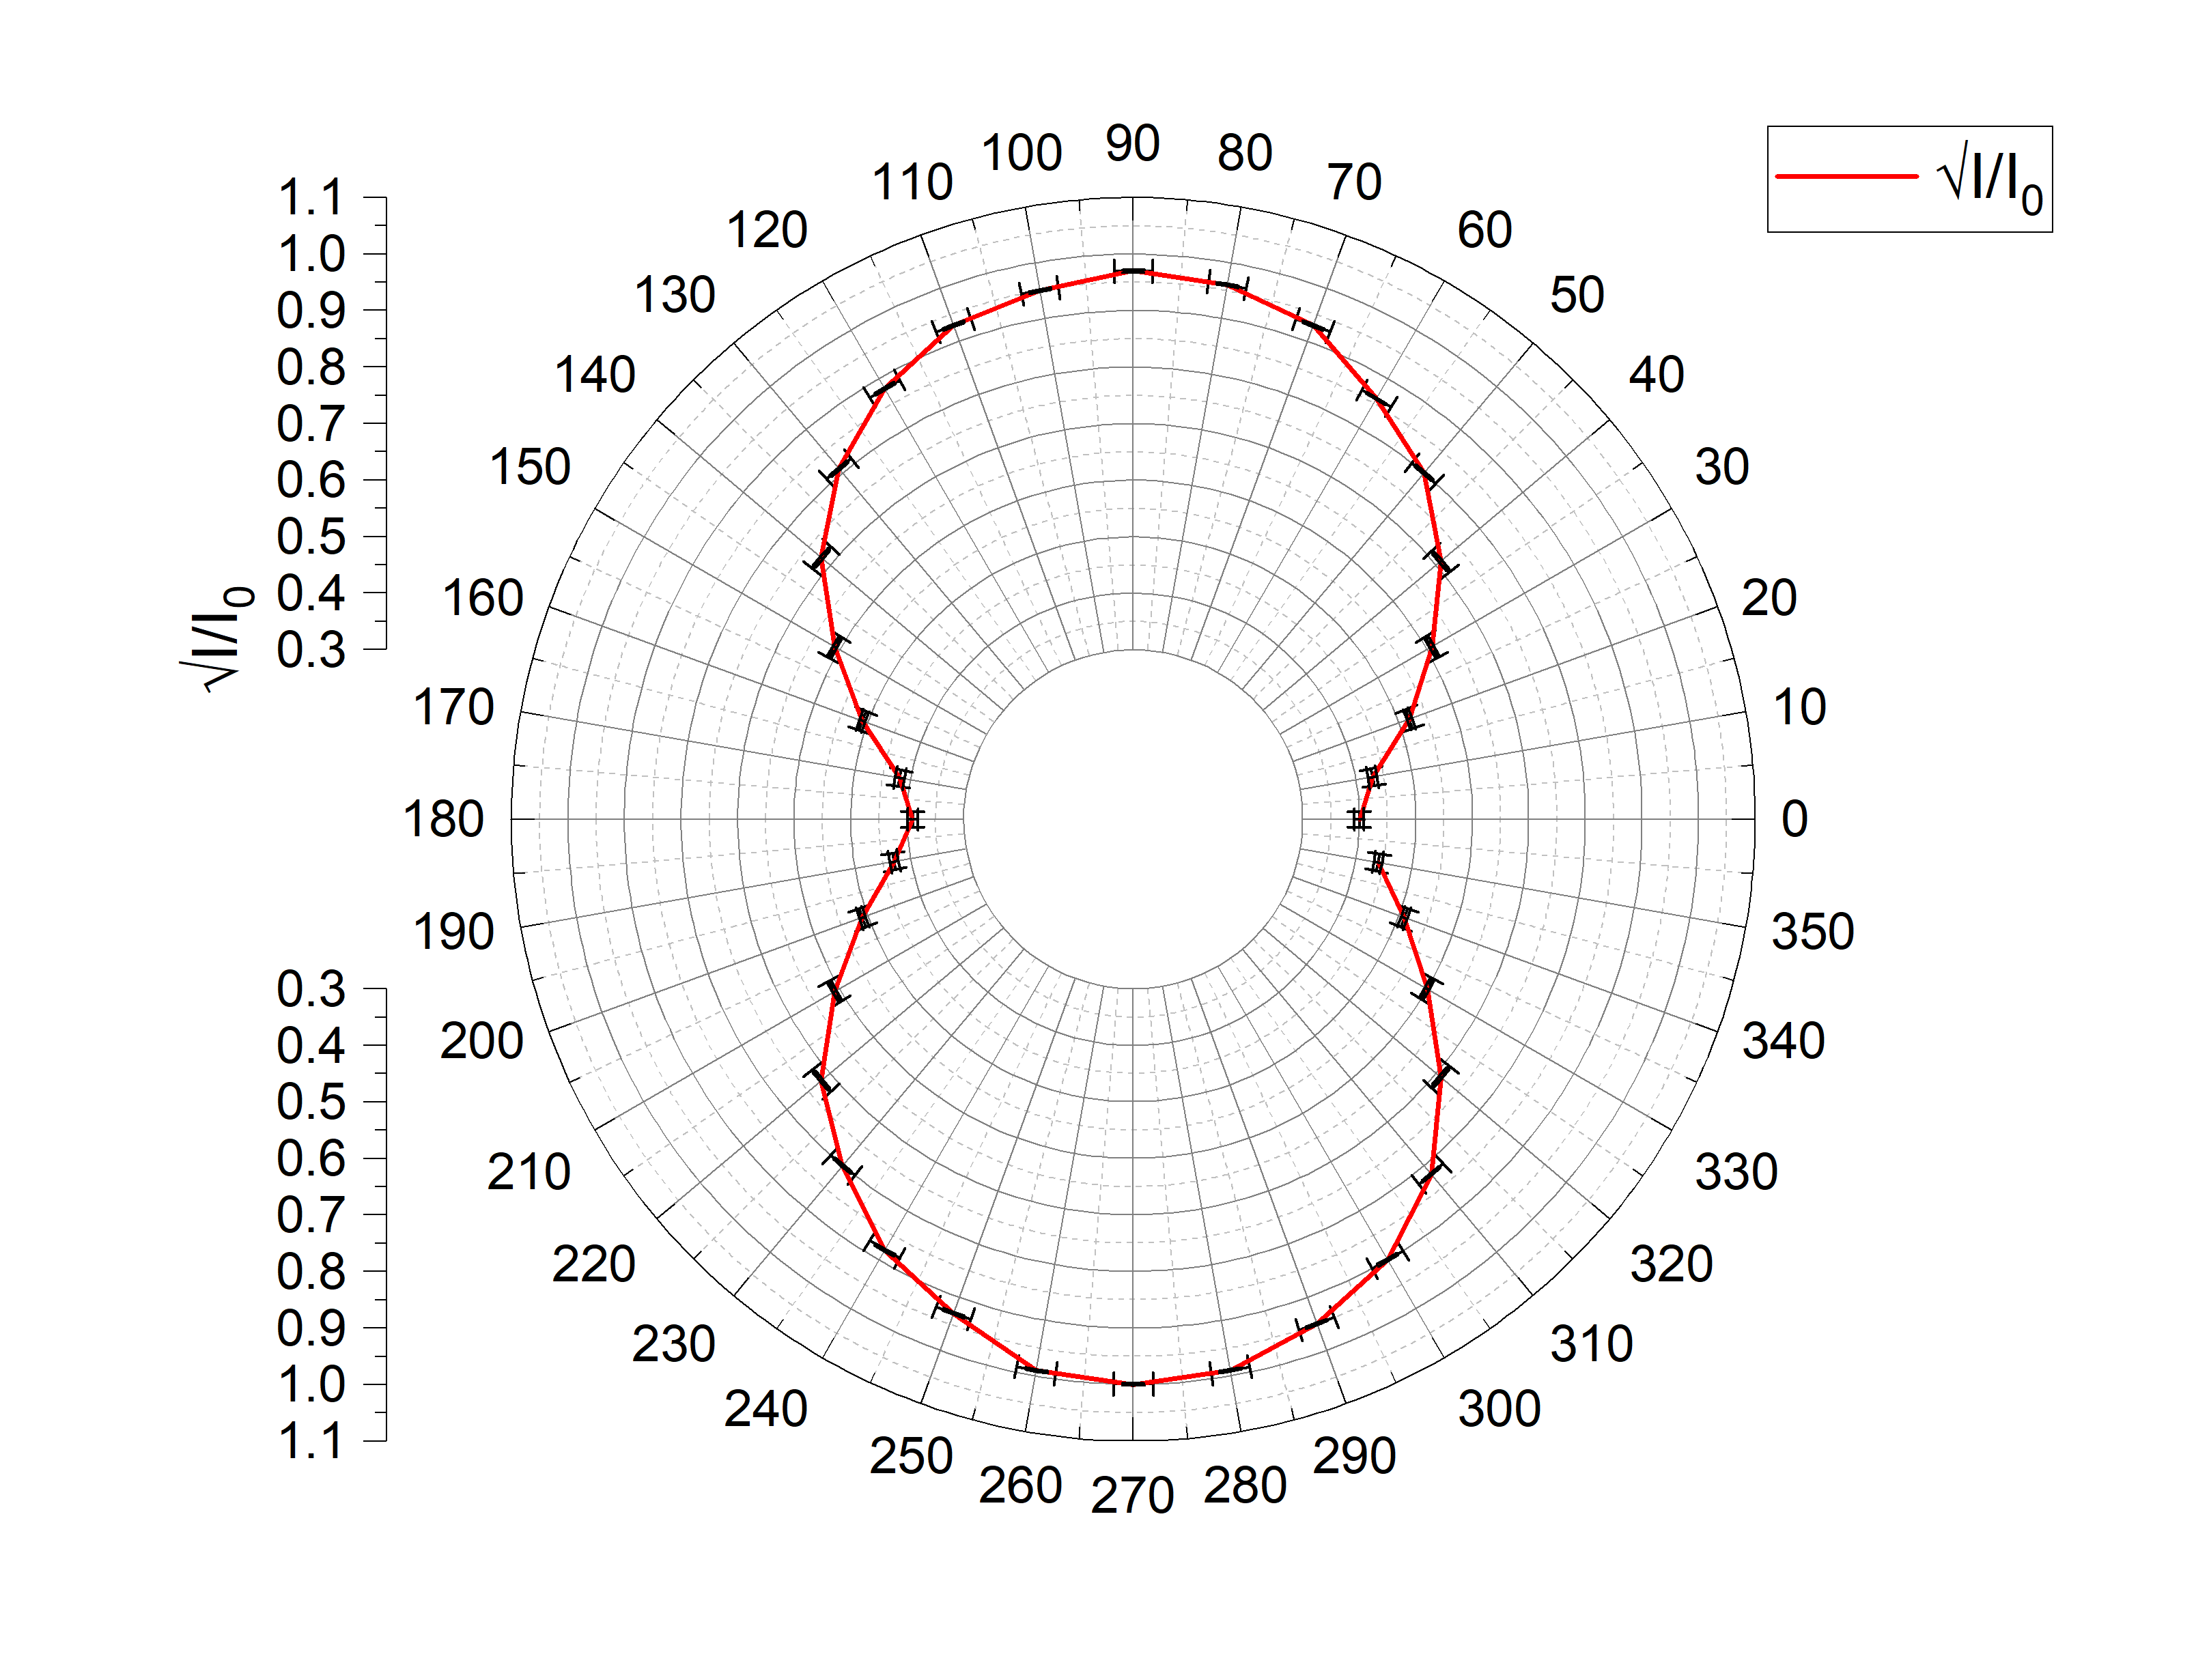
\includegraphics[scale=0.6]{4.png}
\caption{$\sqrt{I/I_0}$ vs. $\theta$ relation in polar coordinate when rotation angle is 20$^\circ$.}\label{Fig20}
\end{figure}


\newpage

\subsubsection{Rotation Angle: 45$^\circ$}

The measurement data for 45$^\circ$ rotation angle of 1/4-wave plate are shown in Table \ref{Table1/445}.  

\begin{table}[H]\centering
\begin{tabular}{cc||cc}
\multicolumn{4}{c}{Rotation angle of 1/4-wave plate: 45$^\circ$}\\
\toprule
\multicolumn{2}{c}{Maximum Electric Current $I_0$} & \multicolumn{2}{c}{0.395 $\pm$ 0.001 [$\mu$A]}\\
\midrule
$\theta\,\,[^\circ] \pm 2[^\circ]$ & $I\,\,[\mu\text{A}] \pm 0.001\,\,[\mu\text{A}]$ & $\theta\,\,[^\circ] \pm 2[^\circ]$ & $I\,\,[\mu\text{A}] \pm 0.001\,\,[\mu\text{A}]$\\
\midrule
0 & 0.566 & 180 & 0.553 \\
10 & 0.572 & 190 & 0.606 \\
20 & 0.568 & 200 & 0.600 \\
30 & 0.573 & 210 & 0.609 \\
40 & 0.596 & 220 & 0.617 \\
50 & 0.624 & 230 & 0.646 \\
60 & 0.614 & 240 & 0.648 \\
70 & 0.627 & 250 & 0.648 \\
80 & 0.664 & 260 & 0.650 \\
90 & 0.664 & 270 & 0.666 \\
100 & 0.646 & 280 & 0.680 \\
110 & 0.624 & 290 & 0.672 \\
120 & 0.633 & 300 & 0.673 \\
130 & 0.635 & 310 & 0.645 \\
140 & 0.654 & 320 & 0.620 \\
150 & 0.646 & 330 & 0.605 \\
160 & 0.627 & 340 & 0.587 \\
170 & 0.602 & 350 & 0.576  \\
\bottomrule
\end{tabular}
\caption{Measurement data for the 1/4-wave plate (rotation angle 45$^\circ$).}\label{Table1/445}
\end{table}

Similarly, $\sqrt{I/I_0}$ is calculated and the results are presented in Table \ref{TableSqrt45}.

\begin{table}[H]\centering
\begin{tabular}{ccc||ccc}
\toprule
$\theta\,\,[^\circ] \pm 2[^\circ]$ & $\sqrt{I/I_0}$ & $\mu_{\sqrt{I/I_0}}$ & $\theta\,\,[^\circ] \pm 2[^\circ]$ & $\sqrt{I/I_0}$ & $\mu_{\sqrt{I/I_0}}$ \\
\midrule
0 & 0.6897 & 0.0003 & 180 & 0.6817 & 0.0003 \\
10 & 0.6933 & 0.0003 & 190 & 0.7136 & 0.0003 \\
20 & 0.6909 & 0.0003 & 200 & 0.7101 & 0.0003 \\
30 & 0.6939 & 0.0003 & 210 & 0.7154 & 0.0003 \\
40 & 0.7077 & 0.0003 & 220 & 0.7201 & 0.0003 \\
50 & 0.7241 & 0.0003 & 230 & 0.7368 & 0.0003 \\
60 & 0.7183 & 0.0003 & 240 & 0.7379 & 0.0003 \\
70 & 0.7259 & 0.0003 & 250 & 0.7379 & 0.0003 \\
80 & 0.7470 & 0.0003 & 260 & 0.7391 & 0.0003 \\
90 & 0.7470 & 0.0003 & 270 & 0.7481 & 0.0003 \\
100 & 0.7368 & 0.0003 & 280 & 0.7559 & 0.0003 \\
110 & 0.7241 & 0.0003 & 290 & 0.7515 & 0.0003 \\
120 & 0.7293 & 0.0003 & 300 & 0.7520 & 0.0003 \\
130 & 0.7305 & 0.0003 & 310 & 0.7362 & 0.0003 \\
140 & 0.7413 & 0.0003 & 320 & 0.7218 & 0.0003 \\
150 & 0.7368 & 0.0003 & 330 & 0.7130 & 0.0003 \\
160 & 0.7259 & 0.0003 & 340 & 0.7023 & 0.0003 \\
170 & 0.7113 & 0.0003 & 350 & 0.6957 & 0.0003\\
\bottomrule
\end{tabular}
\caption{Results for $\sqrt{I/I_0}$ when rotation angle is 45$^\circ$.}\label{TableSqrt45}
\end{table}

Then the relationship of $\sqrt{I/I_0}$ and $\theta$ are plotted in polar coordinate (Figure \ref{Fig45}).

\begin{figure}[H]\centering
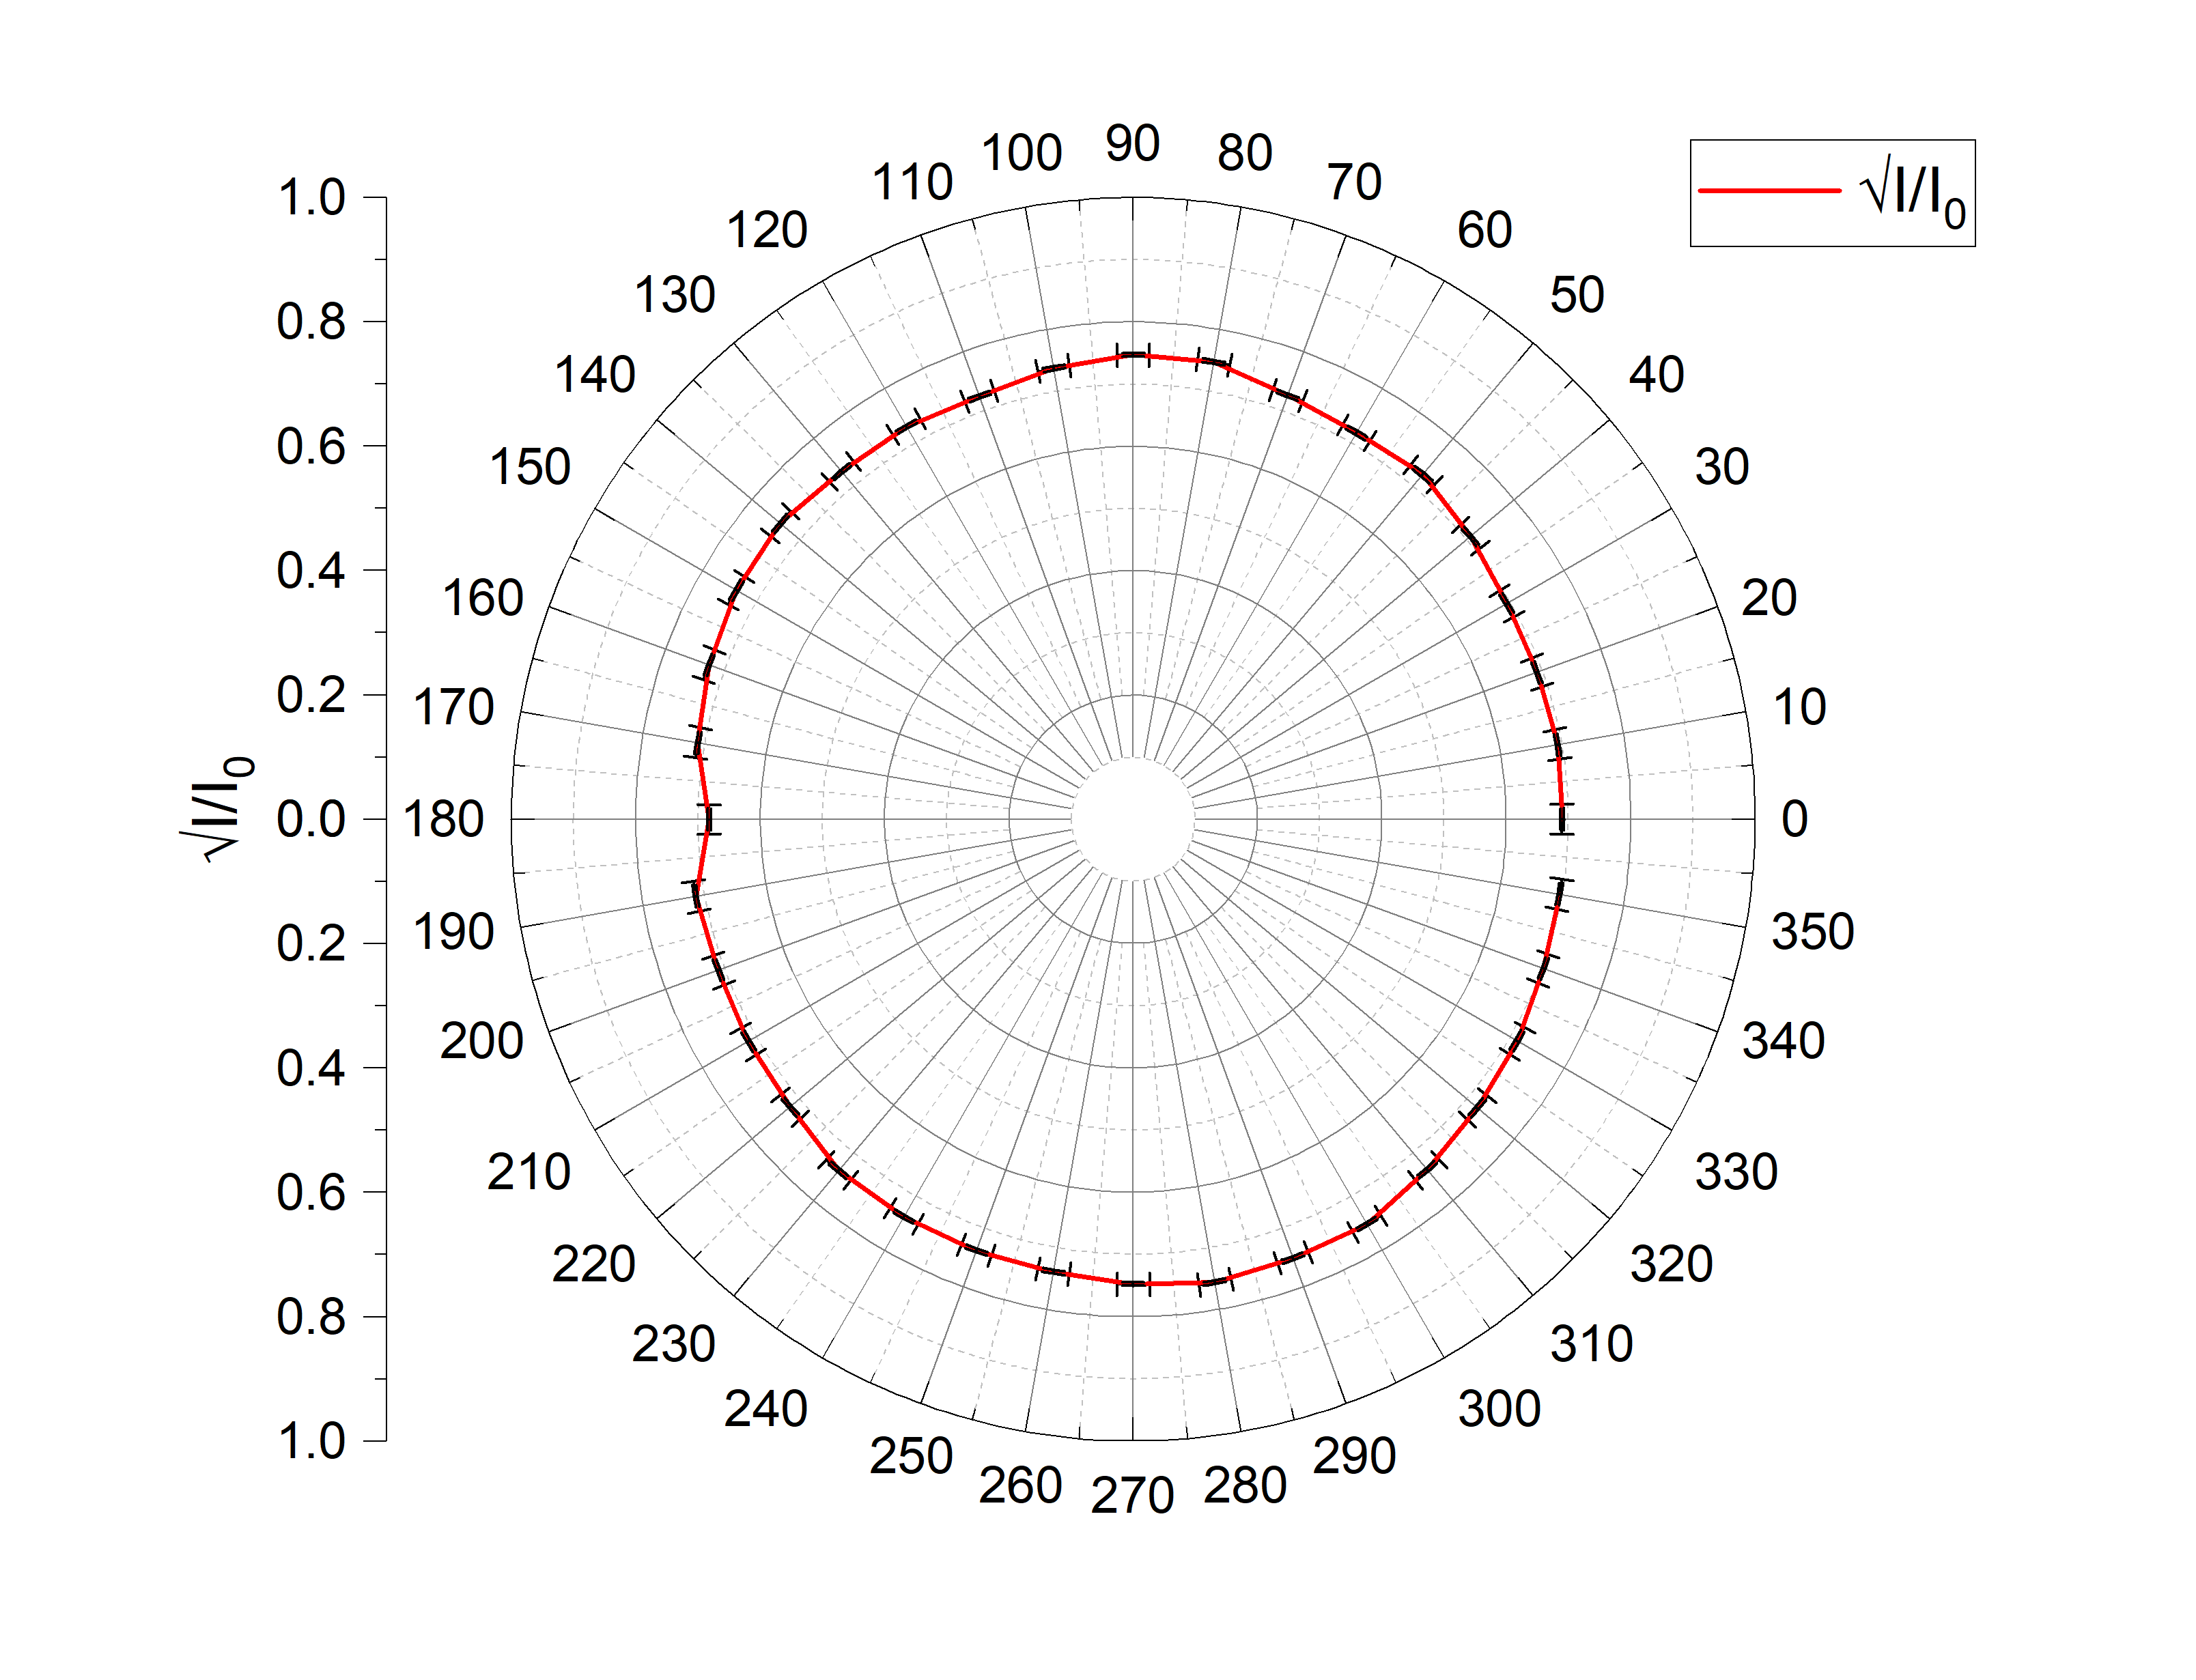
\includegraphics[scale=0.45]{5.png}
\caption{$\sqrt{I/I_0}$ vs. $\theta$ relation in polar coordinate when rotation angle is 45$^\circ$.}\label{Fig45}
\end{figure}

The data is also plotted in Cartesian coordinate and linear fit is performed (Figure \ref{Fig45l}). The slope of the linear fitting is $6 \times 10^{-5} \pm 3 \times 10^{-5}$ with Pearson's r = 0.309.

\begin{figure}[H]\centering
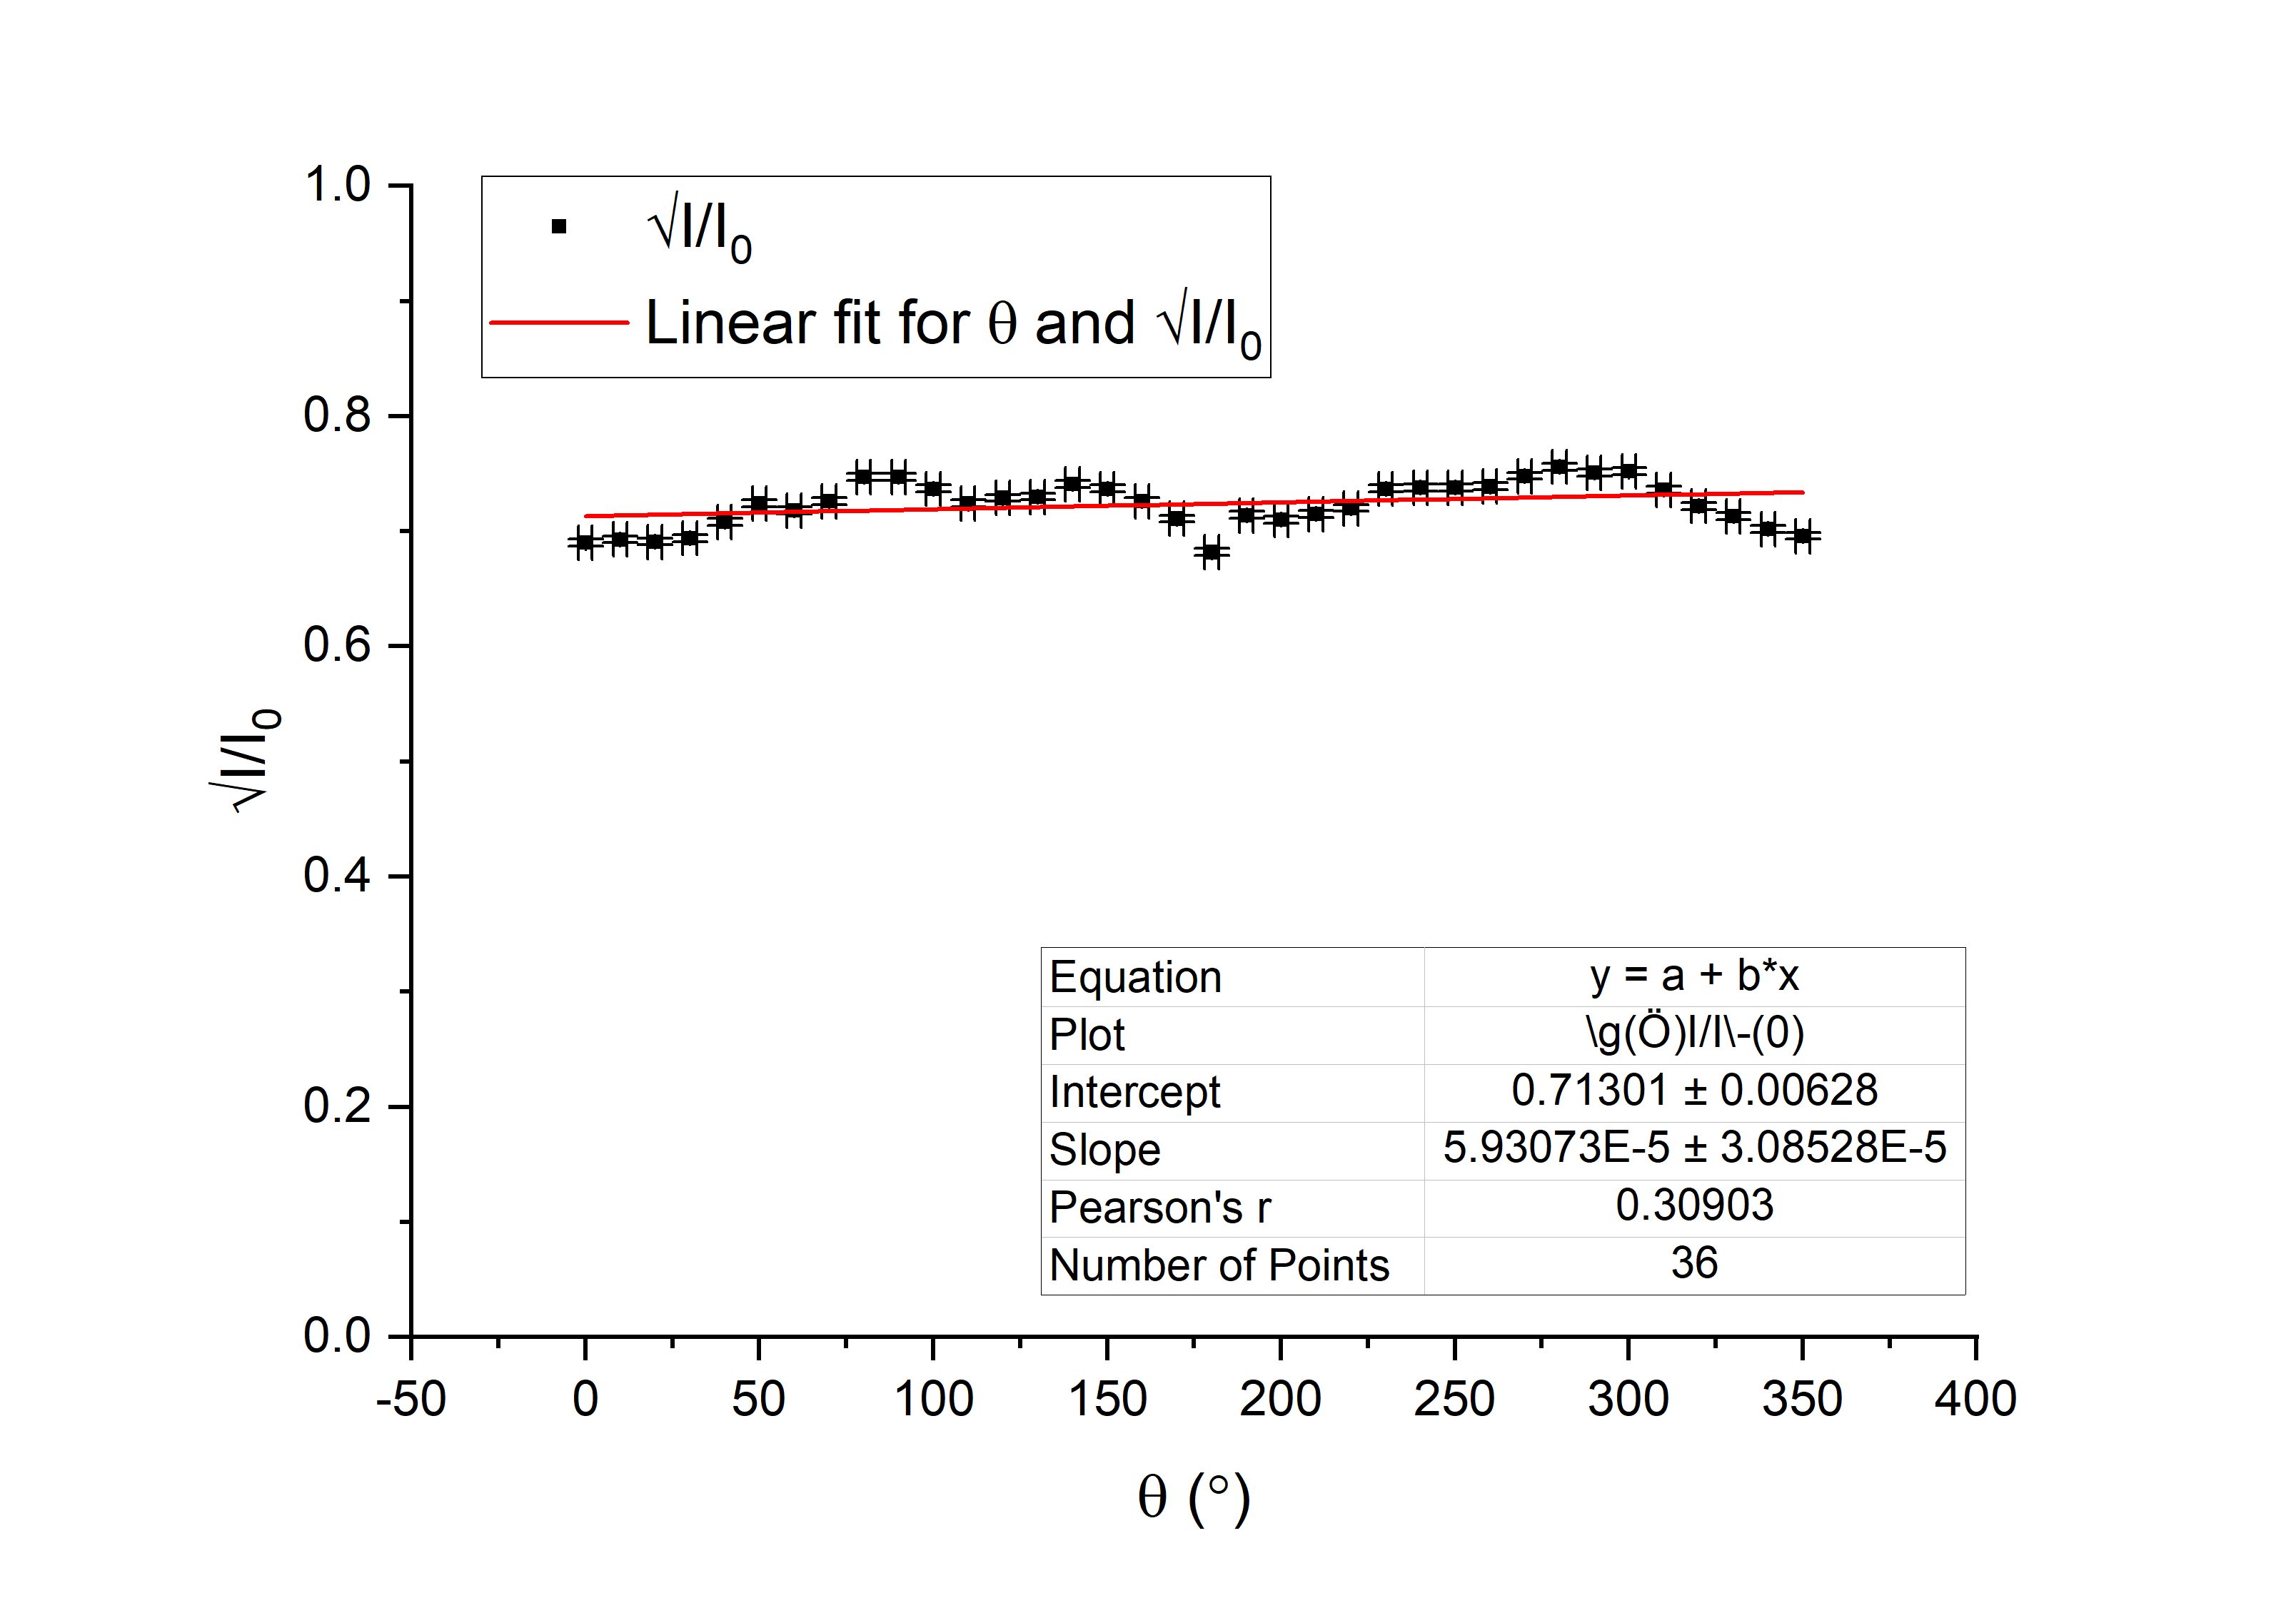
\includegraphics[scale=0.55]{6.png}
\caption{$\sqrt{I/I_0}$ vs. $\theta$ relation in the Cartesian coordinate.}\label{Fig45l}
\end{figure}


\subsubsection{Rotation Angle: 70$^\circ$}

When rotation angle is 70$^\circ$, the data of maximum light intensity are presented in Table \ref{Table70}. The position of this point is marked in blue star in Figure \ref{Fig70}. From the figure, it can be seen that the value of $\theta$ of maximum light intensity of 70$^\circ$ rotation angle is actually symmetric about the origin with that ($\theta = 270^\circ$) of 20$^\circ$. 

\begin{table}[H]\centering
\begin{tabular}{cc}
\toprule
\multicolumn{2}{c}{Rotation angle of the 1/4-wave plate: 70$^\circ$}\\
\midrule
$\theta\,\,[^\circ] \pm 2[^\circ]$ & 90 \\
$I\,\,[\mu\text{A}] \pm 0.001\,\,[\mu\text{A}]$ & 1.111 \\
\bottomrule
\end{tabular}
\caption{Measurement data for the 1/4-wave plate (rotation angle 70$^\circ$).}\label{Table70}
\end{table}

\begin{figure}[H]\centering
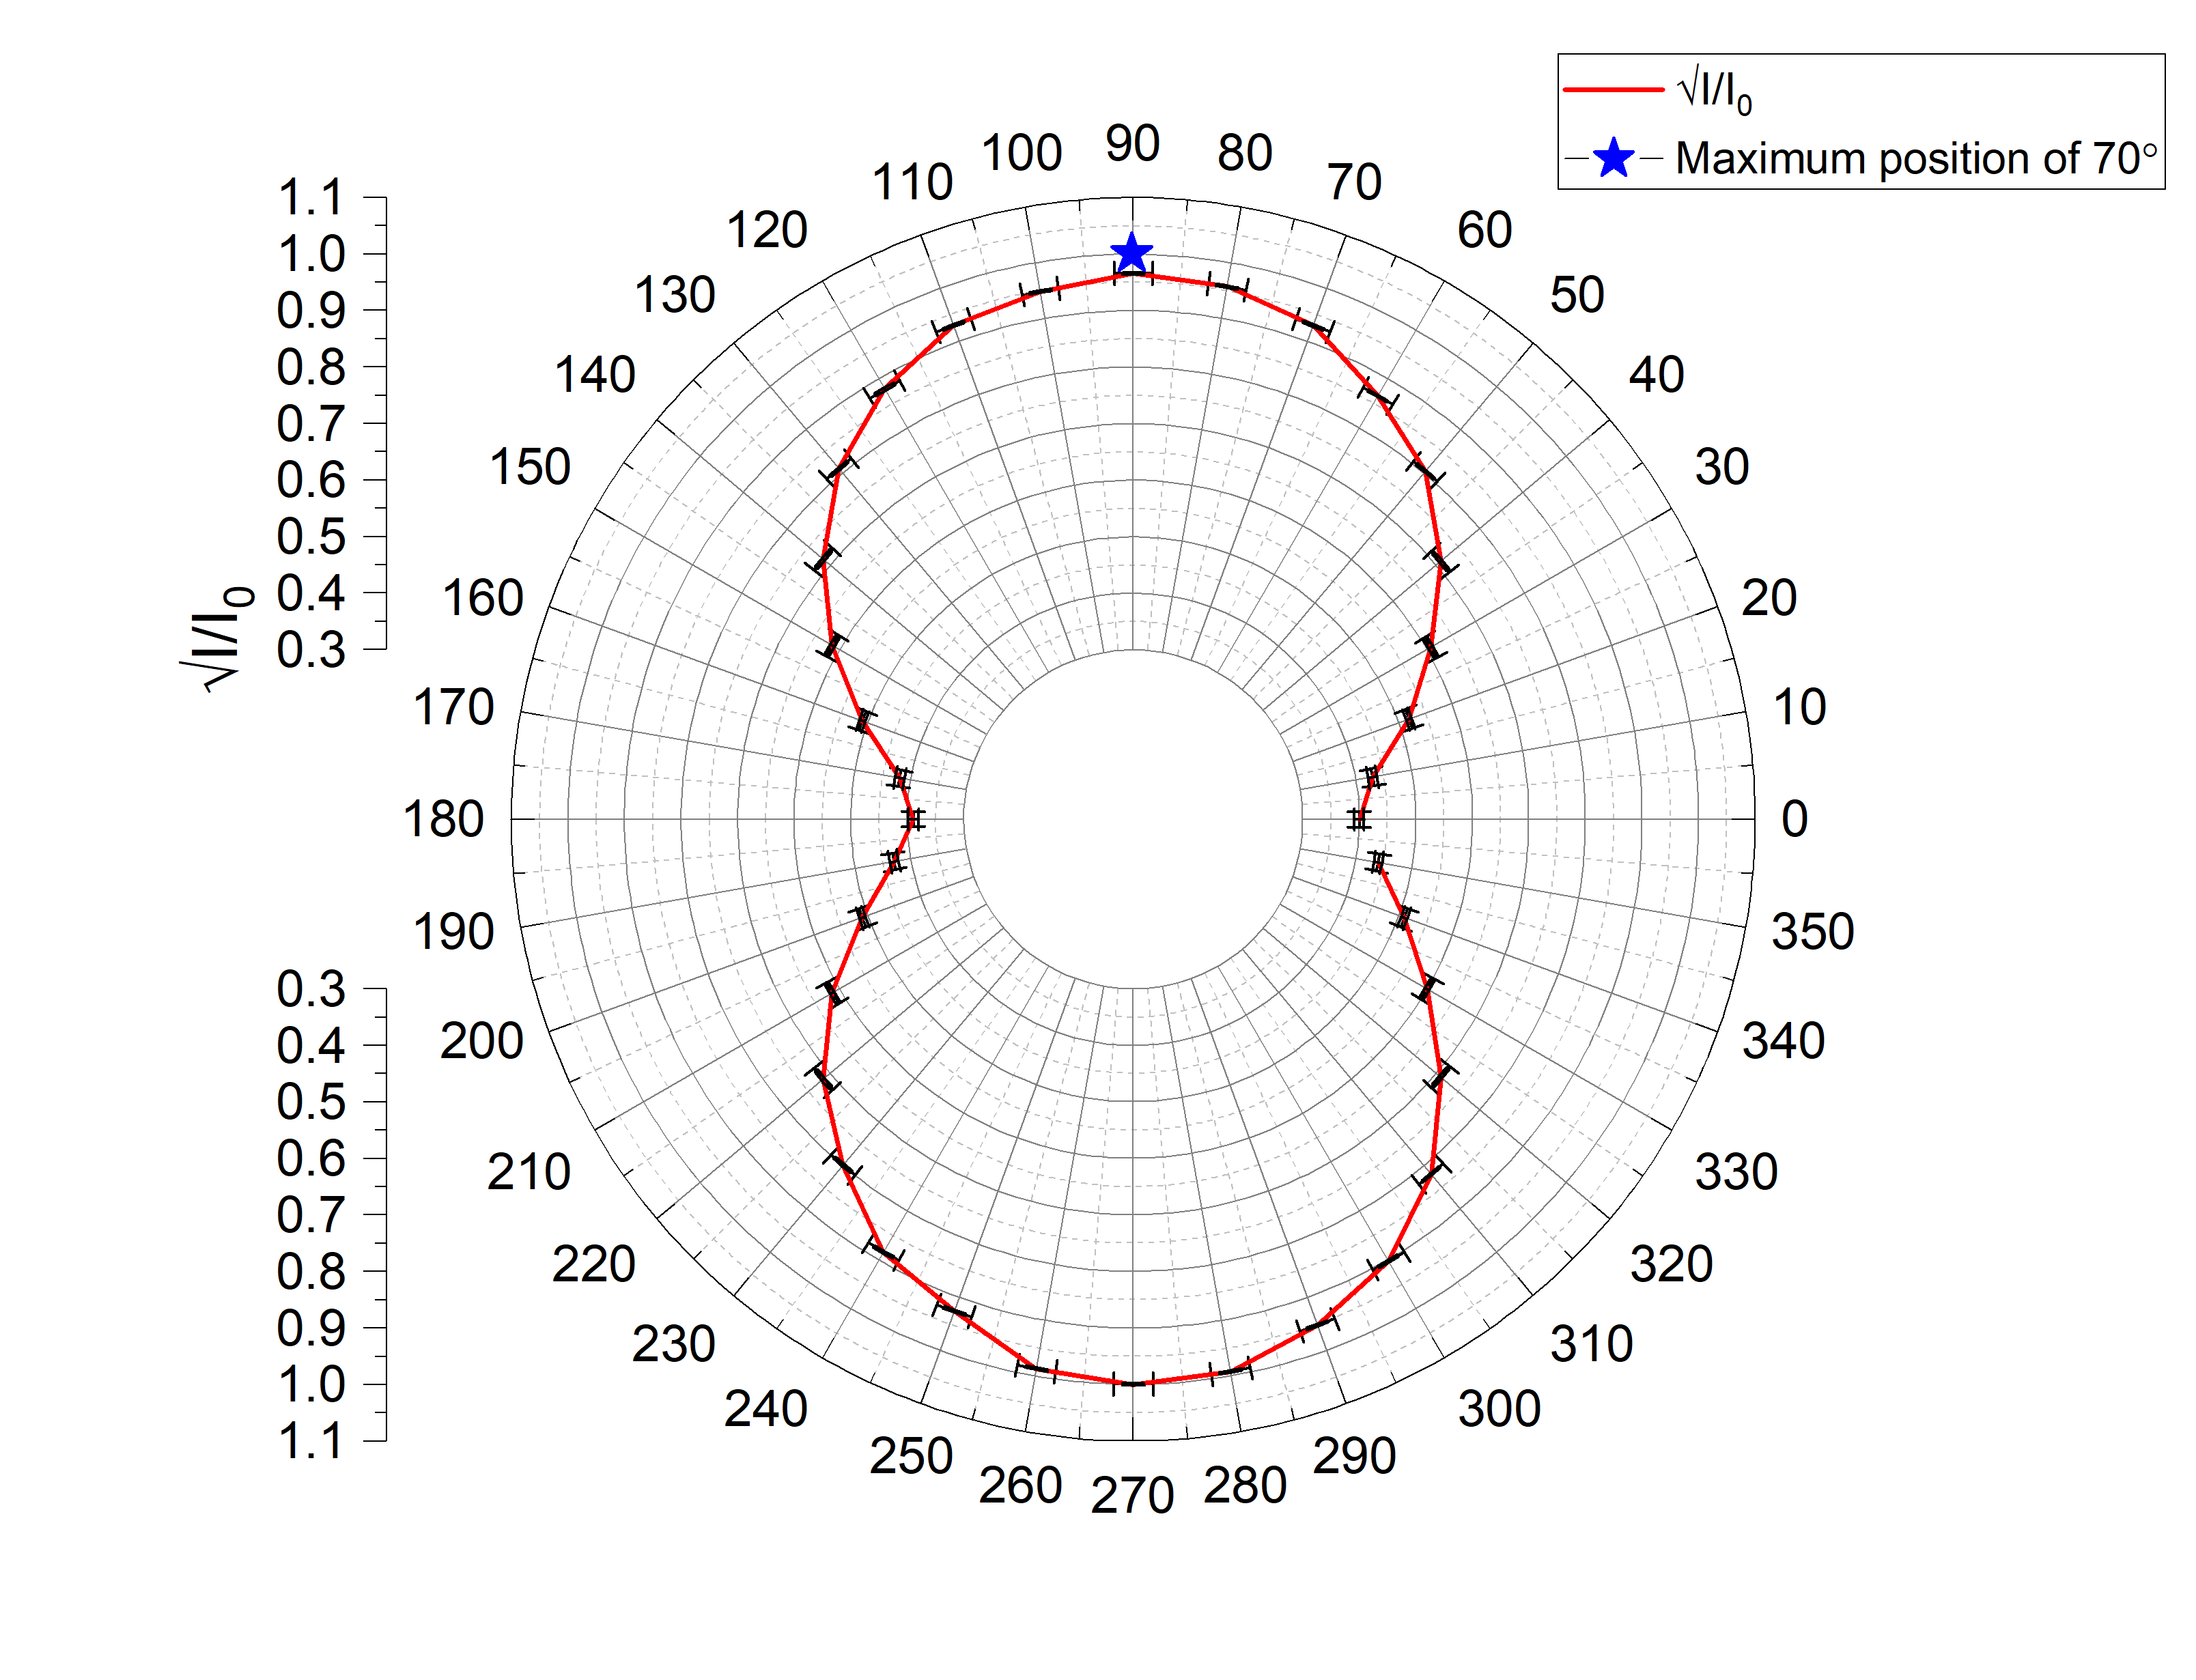
\includegraphics[scale=0.6]{7.png}
\caption{$\sqrt{I/I_0}$ vs. $\theta$ relation in polar coordinate when rotation angle is 20$^\circ$, together with the maximum point of rotation angle 70$^\circ$(marked in blue star).}\label{Fig70}
\end{figure}


\section{Discussion and Conclusions}

\subsection{Demonstration of Malus' Law}

The slope of the fitting for $I/I_0$ v.s. $cos^2\theta$ is 0.988 $\pm$ 0.014 and the Pearson's r is 0.996, which is very close to 1. This indicates a strong linear proportional relationship between the two values. Theoretically, by Eq. \ref{eq.Malus}, the slope should be
$$\frac{I/I_0}{\cos^2\theta} = 1,$$
Therefore, the deviation from theoretical value is
$$u_r = \frac{1-0.988}{1} \times 100\% = 2\%.$$
Which is relatively small and can be used to verified Malus's Law.

\subsection{Linearly Polarized Light and the Half-wave Plate}

The slope of the linear fit for $\Delta\theta$ v.s. $\theta$ is $1.91 \pm 0.05$ and the Pearson's r is 0.999. Theoretically, the rotation angle of the polarization axis should be twice of the origin angle for a half-wave plate. Therefore the theoretical value of the slope of the linear fitting should be 2. The standard deviation is then
$$u_r = \frac{2-1.91}{2}\times 100\% = 5\%.$$ 
Which is relatively small and it can be said that the experimental result fits with the theoretical one.

\subsection{Circularly and Elliptically Polarized Light and the 1/4-wave Plate}

In this section, we mistakenly treated the extinction angle $90^{\circ}$ as $0^{\circ}$. Therefore, all the curves should be rotated for $90^{\circ}$ to correct the mistake. The corrected figures are shown below.

\begin{figure}[H]
\centering
\subfigure[Correction: $\sqrt{I/I_0}$ vs. $\theta$ relation in polar coordinate when rotation angle is 0$^\circ$.]{
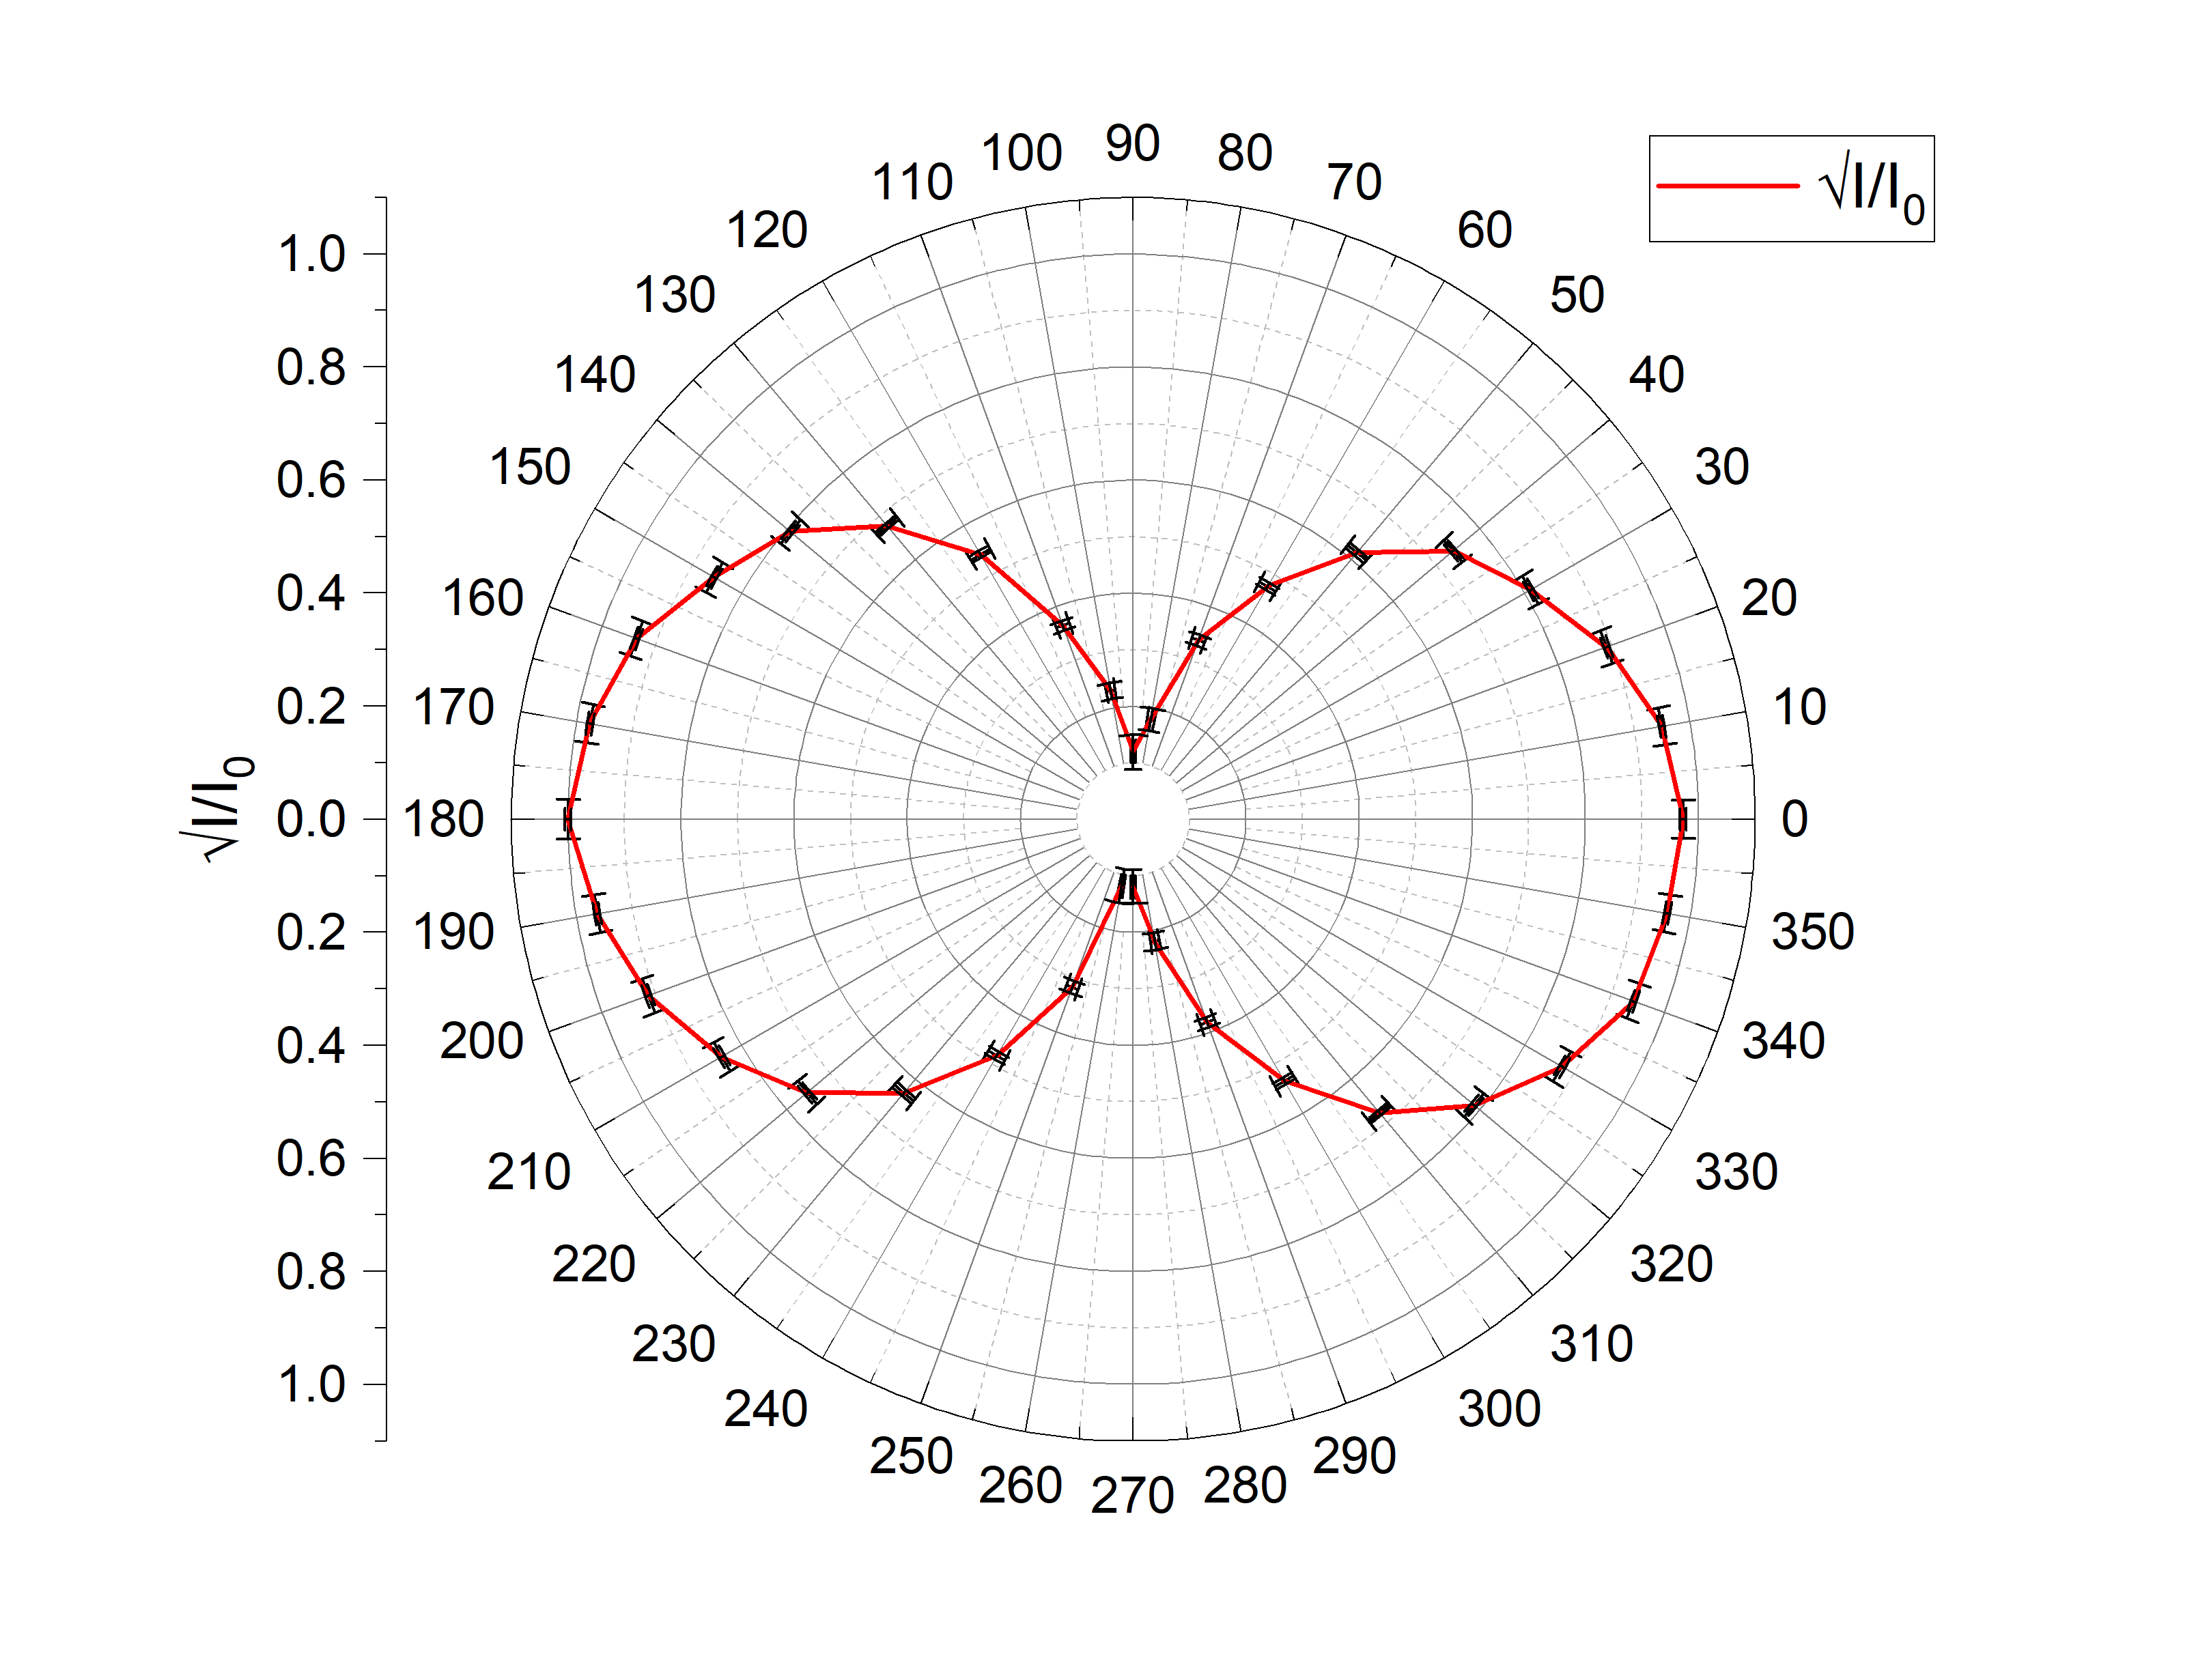
\includegraphics[width=3in]{0.png}\label{a}
}%
\subfigure[Correction: $\sqrt{I/I_0}$ vs. $\theta$ relation in polar coordinate when rotation angle is 20$^\circ$.]{
\centering
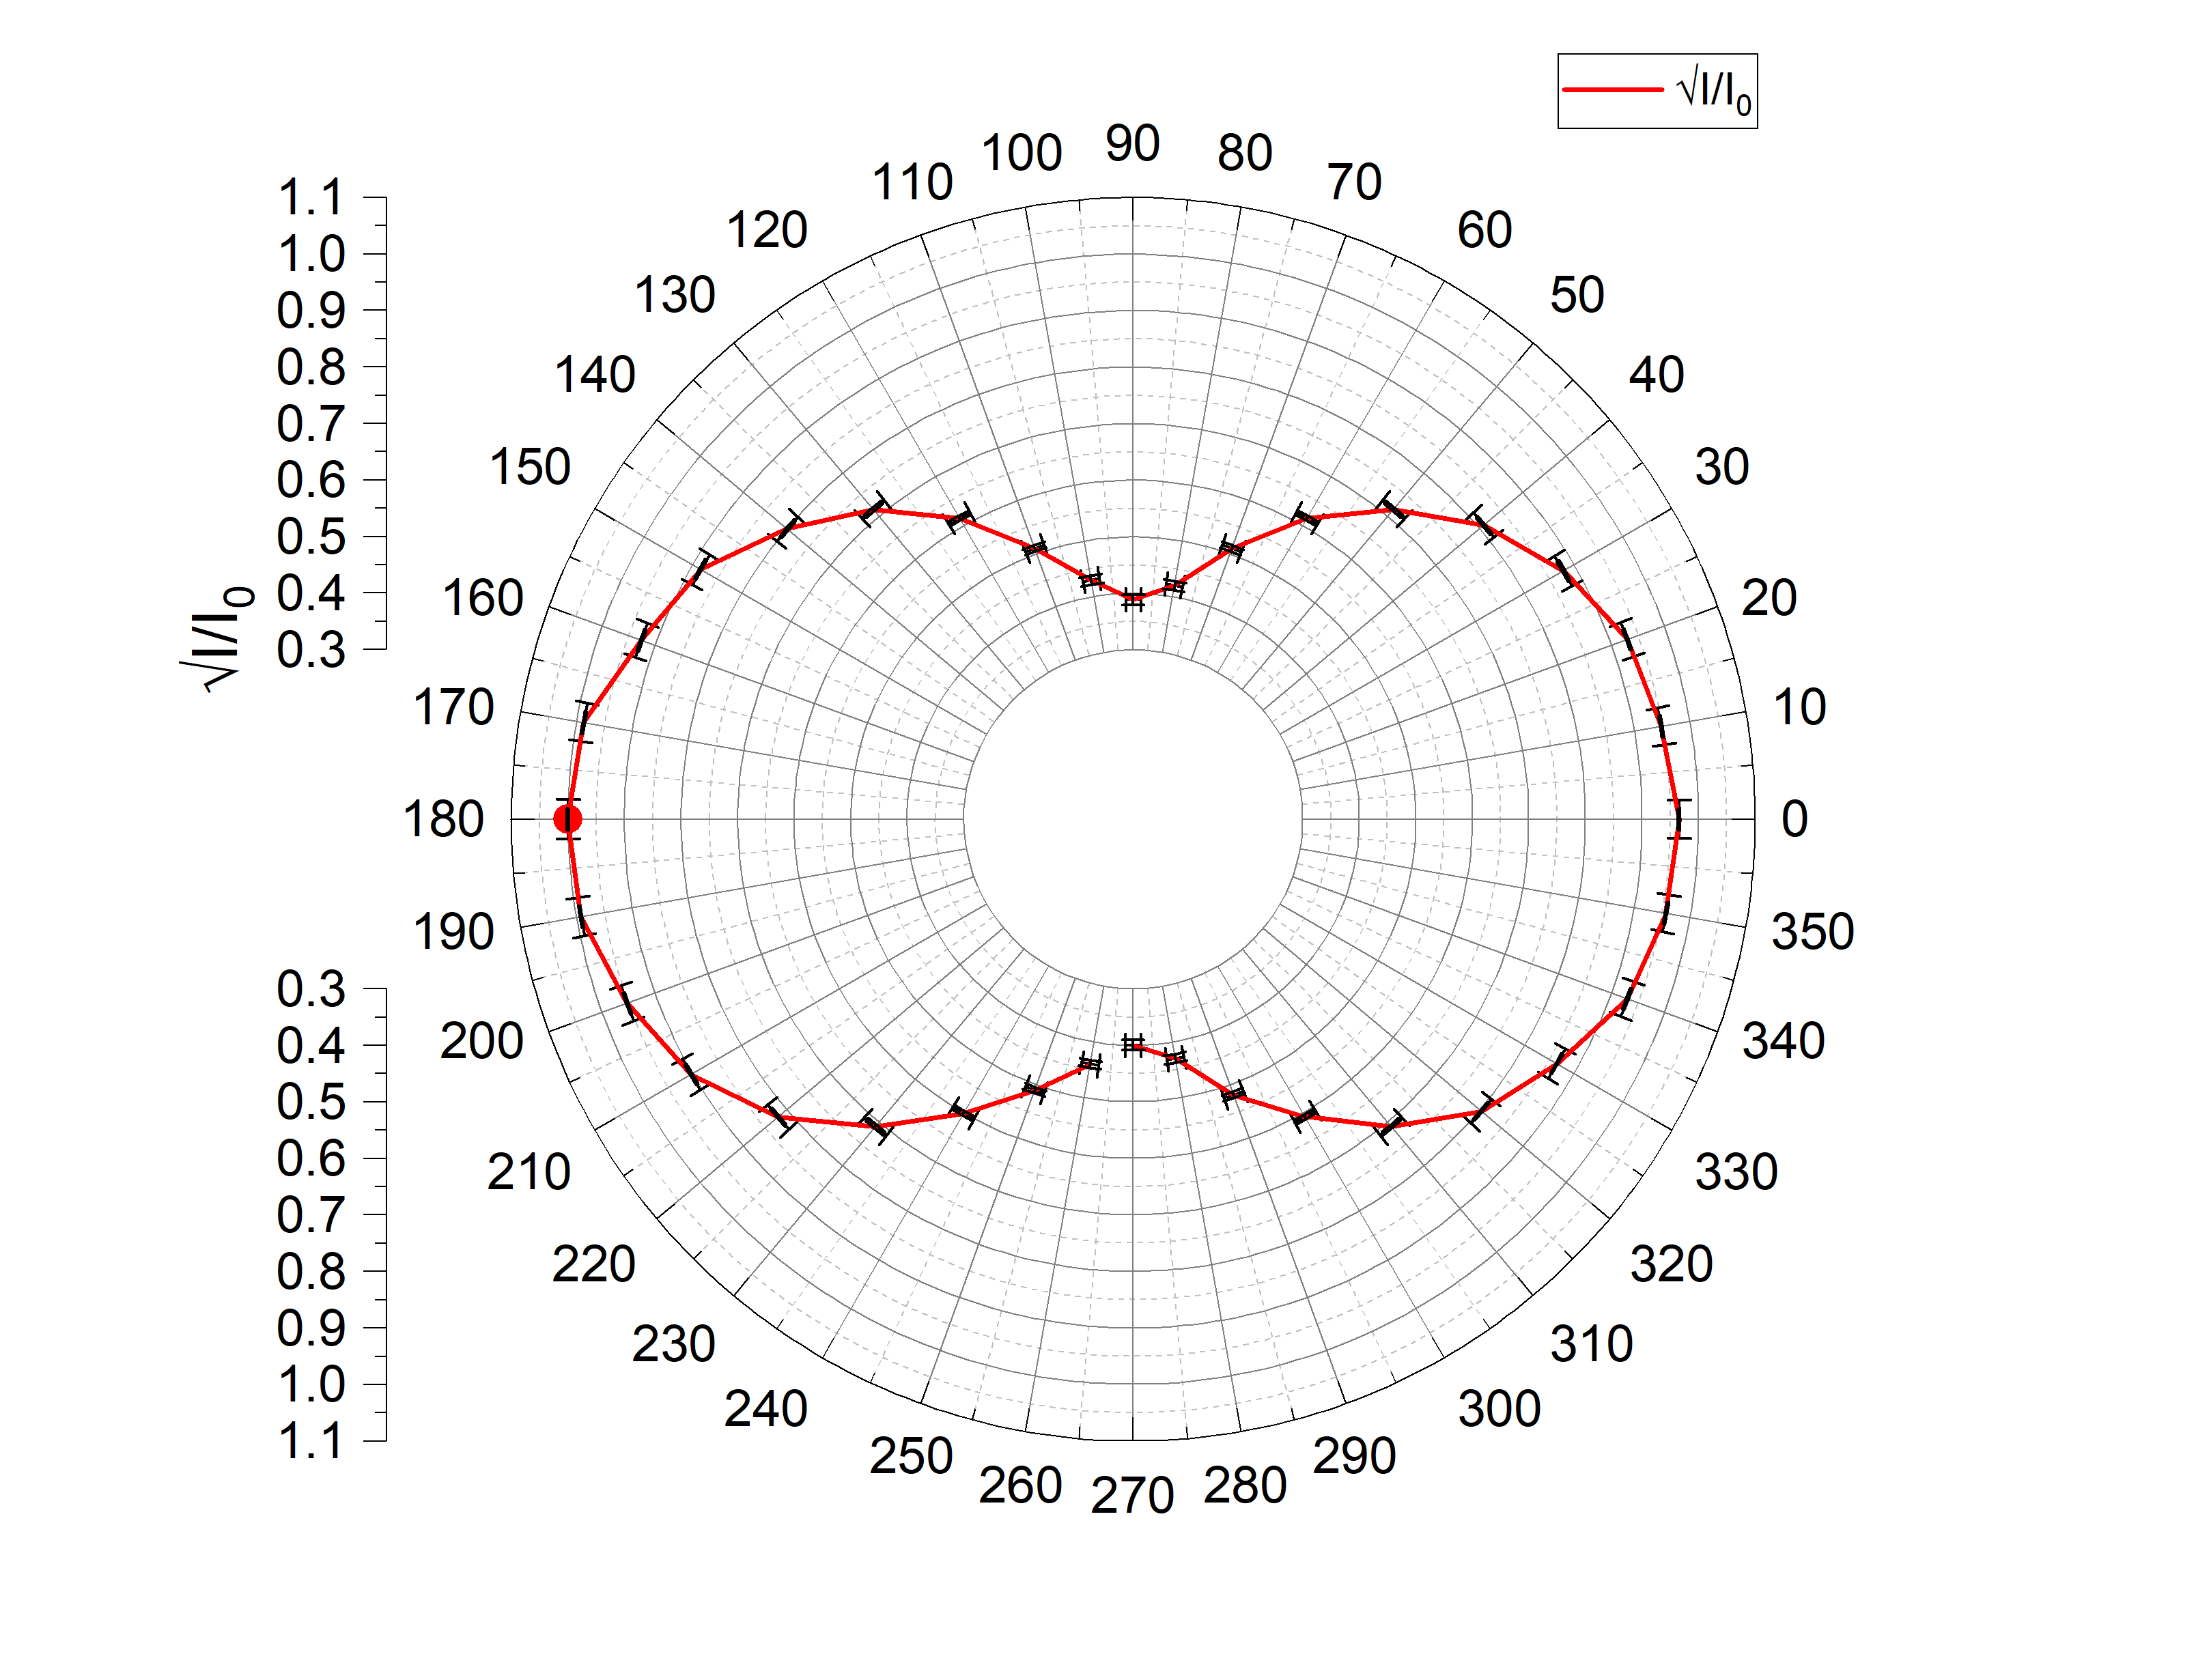
\includegraphics[width=3in]{00.png}\label{b}
}%

\subfigure[Correction: $\sqrt{I/I_0}$ vs. $\theta$ relation in the polar coordinate when rotation angle is 45$^\circ$.]{
\centering
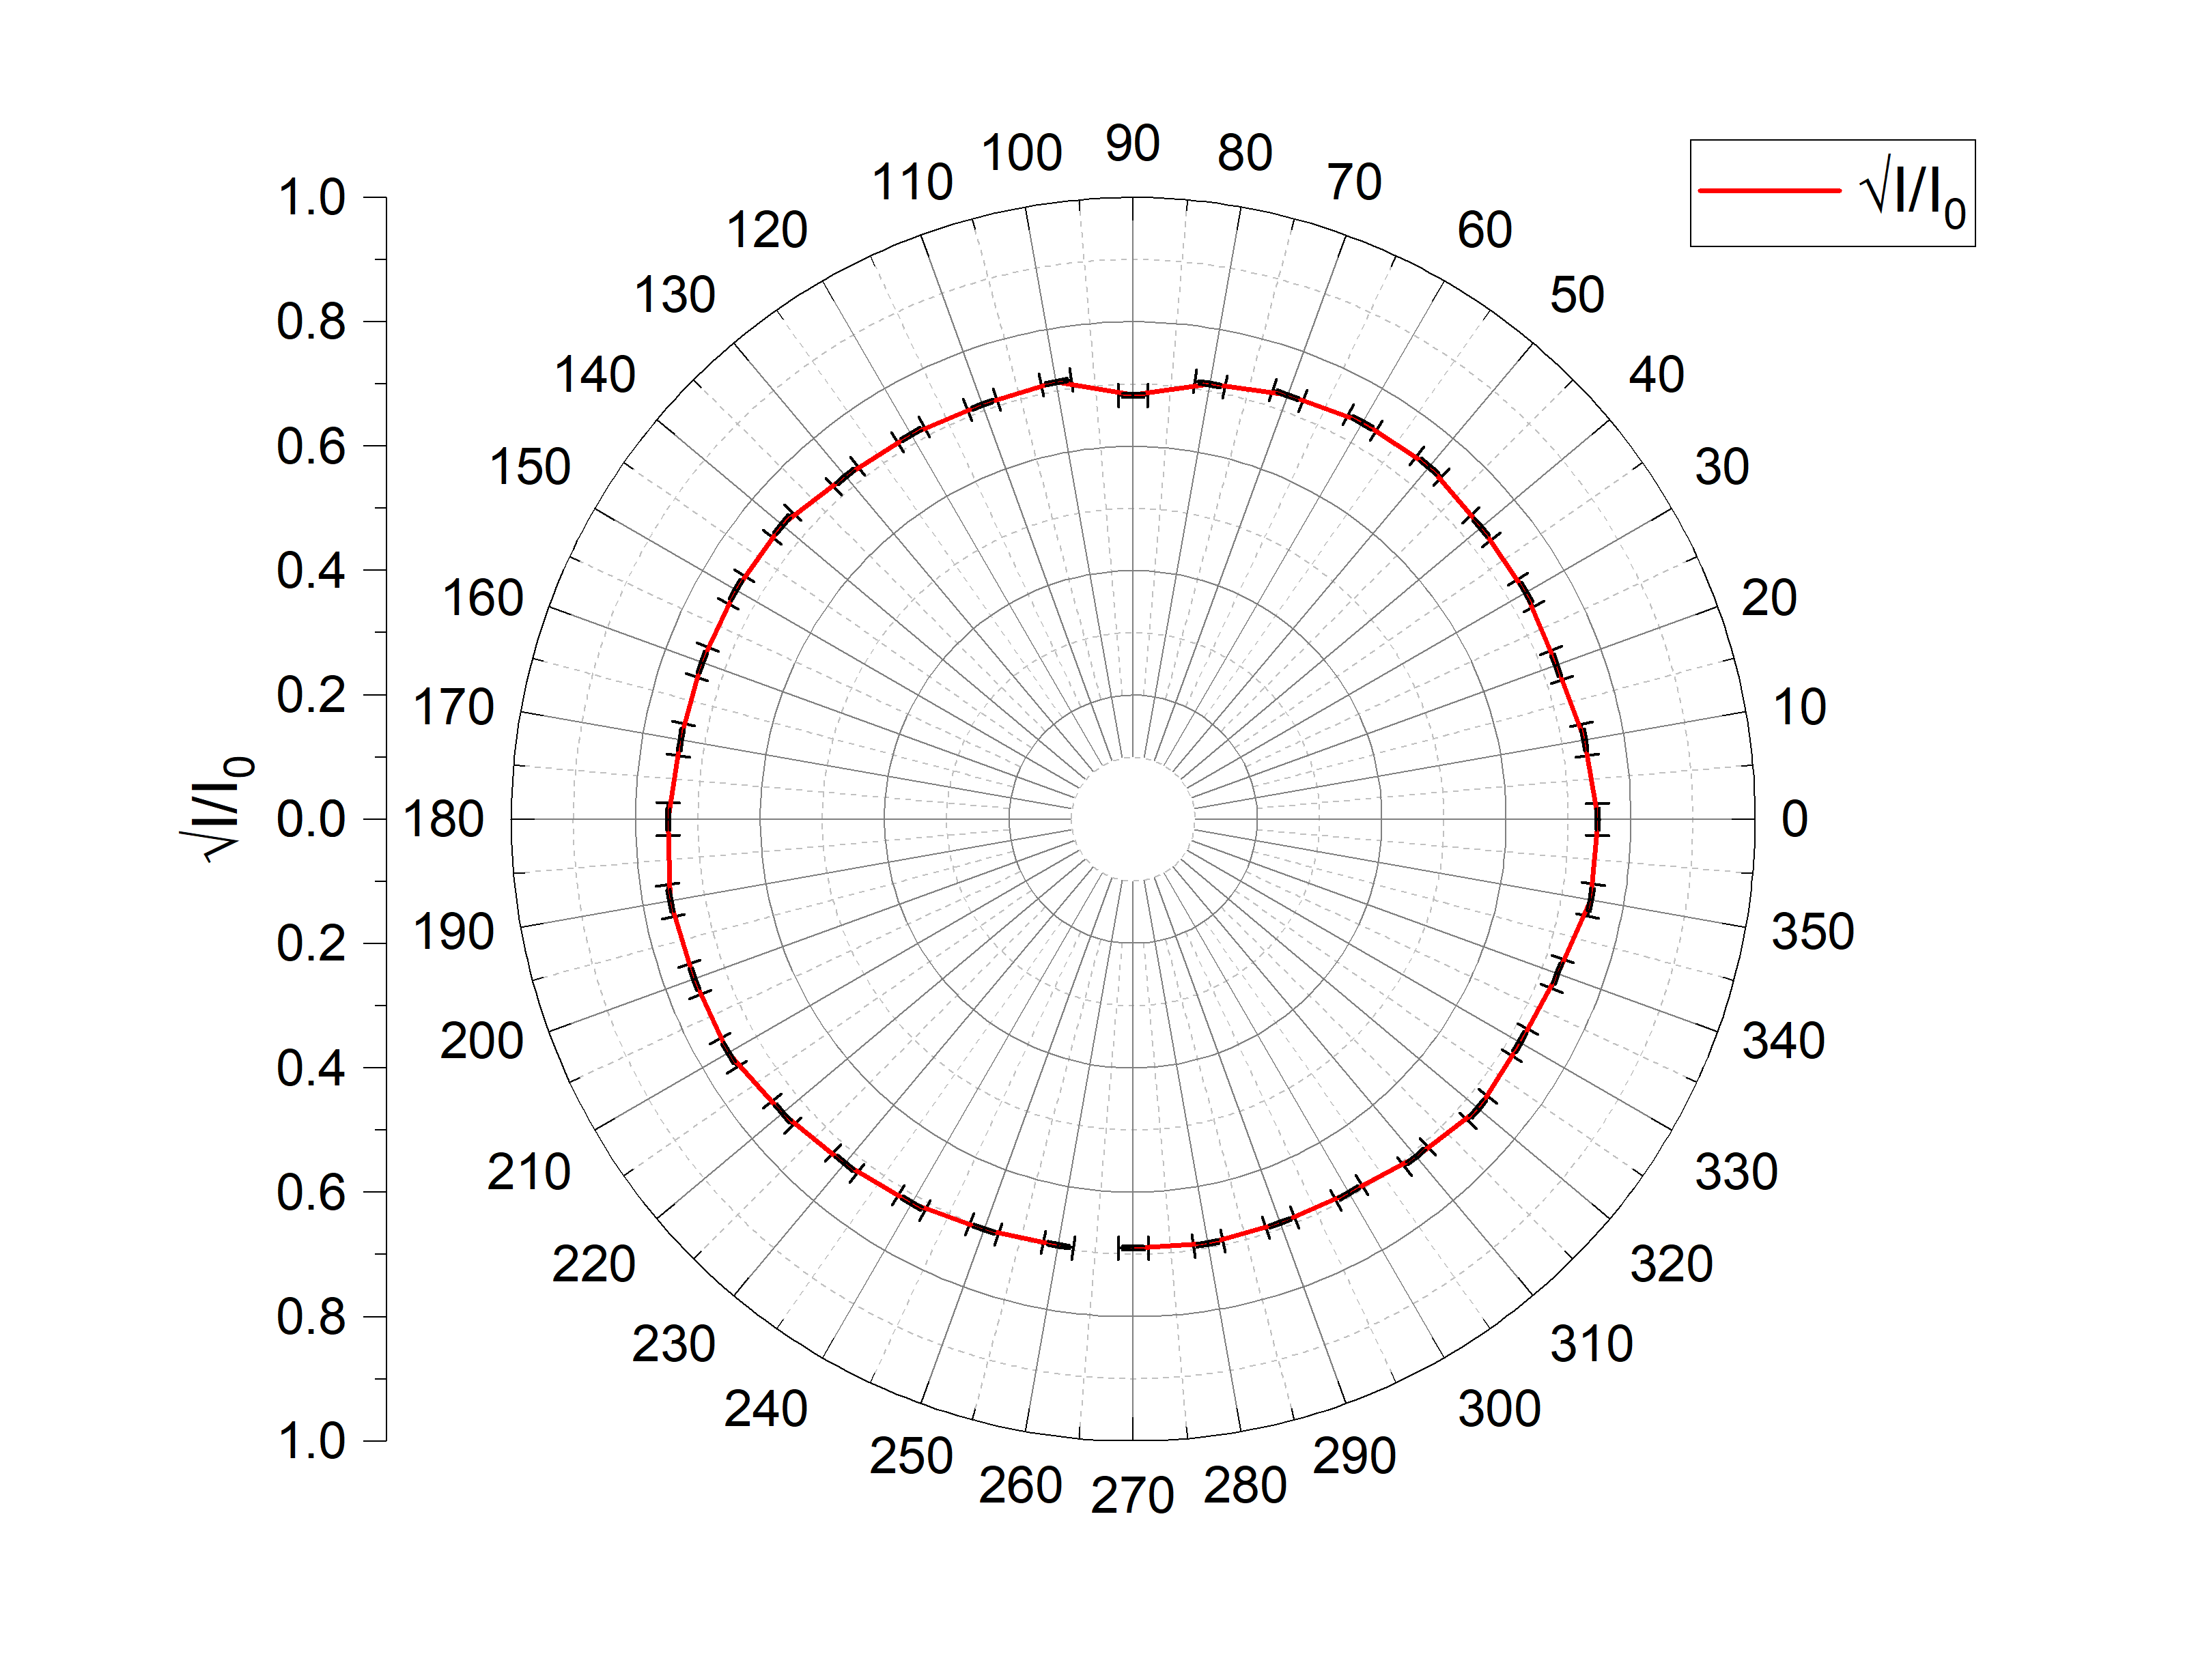
\includegraphics[width=3in]{000.png}\label{c}
}%
\caption{Corrected versions of the figure of $\sqrt{I/I_0}$ vs. $\theta$ }
\end{figure}

\subsubsection{Rotation Angle: 0$^\circ$}

From Table \ref{Table1/40} and Figure \ref{a}, it can be found that the maximum light intensity is at about $\theta = 0^\circ$. This suggests that polarizing axis is in parallel with the optical axis of the plate.

\subsubsection{Rotation Angle: 20$^\circ$}

From Table \ref{Table1/420} and Figure \ref{b}, it can be found that the 
maximum light intensity is still at about $\theta = 0^\circ$. However, according to [1], the angle of maximum light intensity should be $20^{\circ}$, which has relatively big deviation from the experimental one. 
Here are the possible reasons for the error:
\begin{enumerate}
\item Since the rotation angle is only determined by naked eye, and the tick marks on the analyzer are thin and small, it is difficult to precisely rotate exactly $10^{\circ}$ every time. According to the provided uncertainty of analyzer ($\pm2^{\circ}$), it is reasonable that after many times of rotations, small errors accumulate to cause this big error.
\item The reading on the  current meter is always unstable, it is hard to determine when the current reaches a certain value, causing mistaken judgement of the initial angle.
\end{enumerate}


\subsubsection{Rotation Angle: 45$^\circ$}

From Table \ref{Table1/445} and Figure \ref{c}, it can be found that the value of $\sqrt{I/I_0}$ hardly changes  when $\theta$ varies. 

In addition, the slope of the linear fit for $\sqrt{I/I_0}$ vs. $\theta$ in Figure \ref{Fig45l} is only $6 \times 10^{-5} \pm 3 \times 10^{-5}$ and the Pearson's coefficient is only 0.309, which is considerably small. This indicates that there may not be an linear relation between $\sqrt{I/I_0}$ and $\theta$, suggesting that the amplitude is possibly a constant. According to the definition of \textit{circularly polarized}, it can be preliminary concluded that when the rotation angle is 45$^\circ$, the light is circularly polarized. 


\subsubsection{Rotation Angle: 70$^\circ$}

From Table \ref{Table70} and Figure \ref{Fig70}, it can be found that the light intensity reaches maximum at  $\theta = 90^\circ$. It is symmetric about the origin with that of 20$^\circ$ rotation angle. Theoretically, the angle of maximum light intensity should be 70$^\circ$. The reasons for this error are similar to that of rotation angle of 20$^\circ$ (see 5.3.2).   

\subsection{Causes for errors and uncertainties}

Other possible causes for errors and uncertainties are listed below:

\begin{enumerate}
\item This experiment is performed in dark environment, so in order to adjust the apparatus, torch is needed. However, the light from the torch may possible interfere the light intensity detection.
\item On the other hand, the dark environment adds more errors to the readings by naked eyes.
 \item The  scale on the optical elements are not so precise, with uncertainty $2^\circ$, which results in a relatively large errors accumulatively.
\end{enumerate}

\subsection{Suggestions}

Use digital scale to measure the angle of rotation. This not only minimizes the occasional errors but allows the experiment to be performed in a completely dark environment.

\subsection{Conclusions}
In this lab, the polarization phenomenon of light is studied and Malus' law is verified. The working mechanism of half- and quarter-wave plates is also studied. Although the results of circularly polarized light are not accurate due to mistaken operations, the general trend can be verified.

\begin{thebibliography}{1}

\bibitem{manual} VP241 Exercise 4: Polarization of Light, Department of Physics, Shanghai Jiaotong University.

\end{thebibliography}

\newpage

\appendix

\section{Measurement Uncertainty Analysis}

\subsection{Demonstration of Malus' Law}

The uncertainty of $\cos^2\theta$ can be calculated as 
\begin{align*}
u_{\cos^{2}\theta}&=\sqrt{(\frac{\partial \cos^{2}\theta}{\partial \theta}u_{\theta})^{2}}\\
&=|-2u_{\theta}\cos\theta\sin\theta |\\
&=|u_{\theta} \sin2\theta|,
\end{align*}
Here $u_\theta = 2[^\circ] = \pi/90$. 
Take $\theta$ = 0 as an example, 
$$u_{\cos^{2}\theta}=|\sin2\theta u_{\theta}|=|\sin({2\times 5^\circ})\times \frac{\pi}{90}|=0.006,$$

The uncertainty of $I/I_0$ is 
\begin{align*}
u_{I/I_{0}}&=\sqrt{(\frac{\partial I/I_0}{\partial I}u_{I})^{2}+(\frac{\partial I/I_0}{\partial I_{0}}u_{I_{0}})^{2}}\\
&=\sqrt{(\frac{u_{I}}{I_{0}})^{2}+(-\frac{I}{I_{0}^{2}}u_{I_{0}})^{2}},
\end{align*}
where $u_I = u_{I_0} = 0.01\,\,[\mu\text{A}]$, $I_0 = 2.00 \pm 0.01\,\,[\mu\text{A}]$. 
Take the second set of data as an example,
$$u_{I/I_{0}}= \sqrt{(\frac{u_{I}}{I_{0}})^{2}+(-\frac{I}{I_{0}^{2}}u_{I_{0}})^{2}}=\sqrt{(\frac{0.01}{2.00})^{2}+(-\frac{1.97}{2.00^{2}}\times 0.01)^{2}}=0.007,$$

The uncertainties results of $\cos^2\theta$ and $I/I_0$ are shown in Table \ref{tab.Malus2} in the \textbf{Result} section.


\subsection{Linearly Polarized Light and the Half-wave Plate}

The uncertainty is the precision of the device, which is 
$$u_\theta = 2^\circ.$$

\subsection{Circularly and Elliptically Polarized Light and the 1/4-wave Plate}

The uncertainty of $\sqrt{I/I_0}$ is
\begin{align*}
u_{\sqrt{I/I_{0}}}&=\sqrt{(\frac{\partial\sqrt{I/I_0}}{\partial I}u_{I})^{2}+(\frac{\partial\sqrt{I/I_0}}{\partial I_{0}}u_{I_{0}})^{2}}\\
&=\sqrt{\frac{1}{4II_0}u_I^2+\frac{I}{4I_0^3}u_{I_0}^2},
\end{align*}
where 

$u_I = u_{I_0} = 0.01\,\,[\mu\text{A}],~I_0 = 1.50 \pm 0.01\,\,[\mu\text{A}]$ for rotation angle of 0$^\circ$, 

$u_I = u_{I_0} = 0.01\,\,[\mu\text{A}],~I_0 = 1.19 \pm 0.01\,\,[\mu\text{A}]$ for rotation angle of 20$^\circ$, 

$u_I = u_{I_0} = 0.001\,\,[\mu\text{A}],~I_0 = 0.680 \pm 0.001\,\,[\mu\text{A}]$ for rotation angle of 45$^\circ$. 

Take the first set of data in rotation angle of 0$^\circ$ as an example,
$$u_{\sqrt{I/I_{0}}}=\sqrt{\frac{1}{4\times 0.02 \times 1.50} \times 0.01^2+\frac{0.02}{4\times 1.50^3}\times 0.01^2}=0.03.$$

The uncertainties results of $\sqrt{I/I_0}$ are shown in Table \ref{Table1/40}, Table \ref{Table1/420} and Table \ref{Table1/445} in the \textbf{Result} part following the values of  $\sqrt{I/I_0}$.


\section{Data Sheet}

Please find the original data sheet attached at the end of the report.

\end{document}
